\documentclass[12pt]{article}
\usepackage[margin=1in]{geometry}
\setlength{\parindent}{0in}

\usepackage{amsmath,amsthm,amssymb}
\usepackage{graphicx}
\usepackage[dvipsnames]{xcolor}
\usepackage{enumerate}
\usepackage{multicol}
\usepackage{float}
\usepackage{bm}
\usepackage{url}

\newcommand{\res}{\mathcal{R}} \DeclareMathOperator{\arsinh}{arsinh}
\newcommand{\vi}{\bm{\hat{\imath}}} \newcommand{\vj}{\bm{\hat{\jmath}}} 
\newcommand{\vk}{\bm{\hat{k}}} \newcommand{\grad}{\bm \nabla} 
\newcommand{\divg}[1]{\bm{\nabla} \cdot \bm{#1}} \newcommand{\divgg}{\bm{\nabla} \cdot}
\newcommand{\curl}[1]{\bm{\nabla} \times \bm{#1}} \newcommand{\curll}{\bm{\nabla} \times}
\newcommand{\So}{\hbox{So }} \newcommand{\so}{\hbox{ so }}
\newcommand{\Seethat}{\hbox{See that }} \newcommand{\seethat}{\hbox{ see that }}
\newcommand{\Thus}{\hbox{Thus }} \newcommand{\thus}{\hbox{ thus }}
\newcommand{\For}{\hbox{For }} \newcommand{\for}{\hbox{ for }}
\newcommand{\tIf}{\hbox{If }} \newcommand{\tif}{\hbox{ if }}
\newcommand{\As}{\hbox{As }} \newcommand{\as}{\hbox{ as }}
\newcommand{\with}{\hbox{ with }} \newcommand{\tand}{\hbox{ and }} \newcommand{\Let}{\hbox{Let }}
\newcommand{\del}[2]{\frac{\partial #1}{\partial #2}} \newcommand{\dell}[2]{\frac{\partial^2 #1}{\partial #2^2}}
\newcommand{\dstyle}[1]{$\displaystyle #1$} \newcommand{\vhat}[1]{\bm{\hat{#1}}}
\newcommand{\snote}[1]{ \times 10^{#1}} \newcommand{\deltax}{\delta_x}
\newcommand{\bgath}[1]{\begin{gather*} #1 \end{gather*}}
\newcommand{\bath}[1]{\begin{gather} #1 \end{gather}}
\newcommand{\bgaln}[1]{\begin{align*} #1 \end{align*}}
\newcommand{\baln}[1]{\begin{align} #1 \end{align}}
\newcommand{\batrix}[1]{\begin{bmatrix} #1 \end{bmatrix}}

\newcounter{step}
\newcommand{\nextstep}{\stepcounter{step} {\large \textcircled{\footnotesize \thestep}} }
\newcommand{\footnotett}[1]{\stepcounter{footnote}\footnotetext{#1}}

\newcommand{\civ}{\vhat{c}}
\newcommand{\econ}{\vhat{e}}
\newcommand{\soc}{\vhat{s}}

\usepackage[backend=biber,style=authoryear,sorting=nty]{biblatex}
\setlength\bibitemsep{\baselineskip}
\addbibresource{ref.bib}

\begin{document}
\pagenumbering{gobble}
\begin{center}
\quad \\
\quad \\
\quad \\
\quad \\
\quad \\
\quad \\
\quad \\
\quad \\
\quad \\
\quad \\
\quad \\
\LARGE Votes that Count: Building a Tool to Facilitate Understanding of the Effects of Voting Procedure\\ on Electoral Outcomes\\ \normalsize
\quad \\
\quad \\
Spencer Diamond\\
\quad \\
Director: Dr. Hessam Sarjoughian\\
School of Computing and Augmented Intelligence\\
\quad \\
Second Reader: Dr. Taylor Hines\\
Barrett Honors College\\
\quad \\
\end{center}
\newpage
\tableofcontents
\newpage

\pagenumbering{arabic}
\setcounter{page}{1}
%0000000000000000000000000000000000000000000000000000000000000000000000000000000000
%0000000000000000000000000000000000000000000000000000000000000000000000000000000000
\section{Introduction} \label{Introduction}
%0000000000000000000000000000000000000000000000000000000000000000000000000000000000
%0000000000000000000000000000000000000000000000000000000000000000000000000000000000
\qquad The goal of this project was to develop a prototype for an educational tool that will help users understand how the voting system deployed by a government can affect the outcomes of elections. This tool was developed in Java SE, consisting of a model for the simulation of elections capable of supporting various voting systems, along with a variety of fairness measures, and educational and explanatory material. While a completed version of this tool would ideally be fully self-contained, easily accessible in-browser, and provide detailed visualizations of the simulated elections, the current prototype version consists of a GitHub repository containing the code, with the educational material and explanations contained within this paper. Ultimately, the goal of this project was to be a stepping stone on the path to create a tool that will instill a measure of systemic skepticism in the user; to give them cause to question why our systems are built the way they are, and reasons to believe that they could be changed for the better. \\

\qquad In this paper, we take a focused look at voting procedure, which generally refers to the way people cast votes. While there are countless factors that can have great impacts on elections: voting rights, systemic injustice and bias, the economy, number and location of polling places, mail-in ballots, pre-voting, campaigning, ID laws, etc., none of those factors will be considered for this project. Instead we will be looking at voting systems. In the study of elections, a voting system refers to the method by which votes are cast and counted in an election; it is the name for the mathematical formula that takes all the votes and produces a winner. The purpose of this tool is to show a user how that formula can effect elections, and why that is important. \\

\qquad In a representative democracy, elections are supposed to be the way citizens of a nation project their will onto their government. By electing a representative with similar values, citizens should be able to steer the government toward their interests; or at least that is what the voting public generally understands as point of an election \parencite{przeworski}. The American National Election Studies is a National Science Foundation funded collaboration between Stanford University and the University of Michigan that has been collecting data on national American elections since the 1950's through independent surveys. In 2012, 78\% of respondents said they trust the federal government either some or none of the time (ANES). Their data also shows that the `trust in government index,' a score calculated from average responses to a few related survey questions, has been trending downward since data collection began, and was at its lowest ever value in both 2018 and 2020 at only 17 out of 100 (ANES). This data set also shows that since 2008, a majority of respondents with strong opinions believed that ``people don't have a say in what the government does," with 61\% of respondents agreeing with that statement in 2020 (ANES). The Comparative Study of Electoral Systems, a large, multi-national data set comprised of over 200 studies in 57 countries over the last 24 years, shows similar trends (CSES). Clearly, our elections are failing to serve their purpose, and the people have noticed. Through this project, I hope to create a tool to introduce the public to one possible remedy to this problem with our democracy: a change in voting system. \\

\qquad Using data from the CSES, Kees Aarts and Jacques Thomassen at the University of Twente were able to show that peoples' satisfaction with a political system was primarily dependent on how representative the elections are perceived to be \parencite{aarts}. Also using CSES data, Christopher Anderson shows that the amount and distinctiveness of options greatly affects voter satisfaction \parencite{anderson}. So by changing to a new voting system, we could not only increase to quality of representation our government provides, but also increase peoples' satisfaction with our political system. Unfortunately, common experience shows that the average voter is often unaware even of the existence of alternative voting systems, let alone the potential benefits of switching.\footnote{While no comprehensive studies exist in this area, CSES data shows that the average voter is fairly uninformed about politics in general. With that data combined with anecdotal evidence provided by many reform advocates, I find this to be a reasonable statement.} In undertaking this project, I hope to help in providing people with the political education needed to make informed decisions about how they want the government to function. \\

\qquad Finally, an important question that must be addressed is: why make this a simulation? Why have I not instead presented this information as a series of mathematical and logical proofs or simply a static set of predefined examples presented in tables and graphs? The primary reason is that many resources of that kind already exist and they are quite lacking in educational value at least for my target users. Rigorous proofs do have a place in this discussion, but they are far too dense to be useful to anyone not already steeped in this field of study. As for static examples, they can be informative to a point, they are really only useful for explaining the basic rules of each system; what they lack is the ability to show a user how a difference in voting system actually changes the political landscape. The secondary reason is that while this project does aim to be a stepping stone on the way to the creation of a full-fledged tool, it also, like any Barrett Thesis, is supposed to be a learning experience for me as well. \\

%0000000000000000000000000000000000000000000000000000000000000000000000000000000000
%0000000000000000000000000000000000000000000000000000000000000000000000000000000000
\section{Scope} \label{Scope}
%0000000000000000000000000000000000000000000000000000000000000000000000000000000000
%0000000000000000000000000000000000000000000000000000000000000000000000000000000000
\qquad The target users of this project, in its current state, are educated adult voters with at least some programming experience. The current target demographic must be restricted in this way because of the prototype nature of the tool at this point. In order to use the program, users need to have some knowledge of and access to GitHub and a Java distribution; they need to be comfortable retrieving code from a GitHub repository, compiling and running the code. Ultimately, the target user base would be anyone with an internet connection and a curiosity about how our leaders are chosen, but for now this document will assume the reader has a relatively high degree of education. \\

\qquad Owing to the sheer complexity within this topic, it is necessary for this project to have a fairly narrow scope. Firstly, this project focused on single-member, non-districted elections only. What this means is that only one winner is elected, and the voters are not divided into multiple blocks; they all vote together. Examples of single-member elections would be a Presidential, Gubernatorial, or single MP election. In reality, non-districted elections are rare, so an example of a districted election would be the American Presidential election, where votes are counted by state instead of nationally. While there are many multi-winner voting systems, and most of the principles that will be discussed later do translate to these kinds of elections, the specifics are much more complex. Because this tool is meant to serve as an introduction to these concepts, that complexity will be detrimental to building understanding, so these kind of elections are excluded from the project. \\

\qquad Secondly, this model is non-interactive. The only contact a user has with the simulation is specifying the input and receiving the output. For the end user, the program is a `black box' of sorts, operating completely independently. While of course the documentation is available so users can understand how the program functions, at no point does the execution of a simulation require (or even accept) any user participation. \\

\qquad Thirdly, each election is deterministic. If two separate elections of the same type are run with the exact same initial conditions, the same winner will be determined every time. While real world elections with actual people are very stochastic (determined by many random factors), with individuals voting according to their changing inclinations, the percentage difference this is likely to cause would be negligible, so for this project it is assumed that each vote is determined without any randomness. To facilitate this determinism, it is assumed that the initial conditions of the simulation constitute a full description of the political landscape; all political information relevant to the model is accounted for. As such, new Political Entities\footnote{Defined below in \S \ref{TheModel}.} can only be created under special circumstances and only in reference to another established Political Entity. \\

\qquad In a few sections of this paper, I will describe a some important aspects of the model that at first glance may seem to push the project outside this stated scope, so, for clarity, I will address them here.\footnote{Other more complex examples of the project scope being abused are discussed in \S \ref{Limitations}.} First, the initial conditions for the model are, by default, mostly randomly generated. It might seem like this would undermine the deterministic nature of the model. However, this randomness happens outside of the model, and only serves as a convenient way of generating the initial conditions. If a user generates one set of random initial conditions and uses them to run two identical elections, they will be returned the same result every time. Second, the process of ``nudging'' voters in between elections \textit{is} stochastic. However, the model only requires that individual elections be fully deterministic. The randomness in the nudging process helps the model to more accurately reproduce expected real world behavior, and because it happens between elections the determinism of the elections is preserved. Lastly, a shrewd reader will notice that the optional primary step that can be added to the model is technically a multi-winner election. However, within the tool this extra step is only ever analyzed as a part of the larger single winner election, so we need not worry about the extra complexity. \\

%0000000000000000000000000000000000000000000000000000000000000000000000000000000000
%0000000000000000000000000000000000000000000000000000000000000000000000000000000000
\section{The Model} \label{TheModel}
%0000000000000000000000000000000000000000000000000000000000000000000000000000000000
%0000000000000000000000000000000000000000000000000000000000000000000000000000000000
\qquad The actual model used in this tool is based on an extension of a system that some may already be familiar with, often called the ``Political Compass.'' This system is based on the juxtaposition of conflicting political positions. It takes the concepts of `Authoritarianism' and `Libertarianism,' and places them at opposite ends of a coordinate axis. Similarly, it takes the fuzzy concepts of political `Left' and `Right,' and places them at opposite ends of another coordinate axis. These two axis are arranged perpendicular to each other, effectively allowing a person's political ideals to be represented as a point in 2D Cartesian coordinates.\footnote{For a contemporary example of this kind of system see politicalcompass.org; for a more historical example see \cite{brysonmcdill}.} This popular conception of a political compass has a few problems. Firstly, the terms Authoritarianism, Libertarianism, Left, and Right are ill-defined and cause a good amount of confusion. For Authoritarianism and Libertarianism, almost all of the confusion can be removed by a simple relabeling. In this model, these terms are replaced with `Hierarchical' and `Individualist,' and the axis they lie on is called the `Civil Axis.' For Left and Right, the problem stems from the fact that there are two different political concepts described with these terms; either someone's economic ideals or their social ideals can be given these labels, and without specifying which is being talked about this introduces alot of ambiguity. To remedy this issue, this model extended this system into the third dimension by splitting this axis in two, with a new `Economic Axis' labeled with `Socialism' and `Capitalism,' and the new `Social Axis' retaining the `Left' and `Right' labels. To avoid confusion going forward, I will only use the terms Left and Right in their social sense. \\

\qquad In this model, the basic object is called a Political Entity.\footnotett{For clarity, model objects are always capitalized. For example, `voter' refers to the colloquial, real world concept of a person who votes, while `Voter' refers to a Voter object in the model.} In general, a Political Entity is just something that can have a concrete position in the coordinate system we have constructed. Because we have a 3D Cartesian coordinate system, we can easily represent a Political Entity as a 3D vector with Civil, Social, and Economic components. Less familiar readers my be more comfortable thinking of Political Entities simply as points on a grid, but using a vector representation has many advantages over a point representation.\footnote{Additional explanations of what vectors are, how they work, and what these advantages are can be found in \S \ref{SimulationDetails} and \S \ref{Limitations} if needed.} By representing them as vectors, it is easy to find the relative distance between two Political Entities by finding the magnitude of the difference of the vectors. This relative distance, which I will be calling the `\footnote{This is a nonstandard way to use the word norm. In general, the norm of a vector \textit{is} its magnitude, and it would be improper to refer to the `norm between two vectors.' In this paper, I use the term norm as shorthand for ``the norm of the vector that results when one vector is subtracted from the other." I refrain from using the word distance since we are not dealing with units of length.} ' of two Political Entities, is the principle measure for most interactions in the model. Nearly all Political Entities used in a specific simulation will be generated beforehand and fed in as the initial conditions. However, there are many circumstances where the model will need to add a Political Entity to the simulation. In these cases, that added Political Entity is called a `virtual' Political Entity. The term `virtual' may be a bit confusing, so just think of it as the opposite of `actual.' It just means that this object is a fictitious bookkeeping device. Virtual Political Entities are either removed from the simulation as soon as their function is served, or they can be `persistent,' only being removed at the conclusion of a simulation. Virtual Political Entities are never carried over to a separate simulation. \\

\qquad There are two different kinds of Political Entities: Citizens and Parties. Citizens are Political Entities that directly interact with elections. There are two types: Voters and Candidates. Voters are, predictably, Citizens that vote in elections. For a Voter, their specific placement in the coordinate system represents voting preferences. Candidates are Citizens that can be voted for, and their position represents their platform. The norm between a Voter and Candidate represents that Voter's relative preference for that Candidate, so that the Candidate closest to a Voter would be that Voter's first choice in an election. Voters also have an Approval Radius, and will only consider Candidates within that radius. By comparing the norm of each Voter with each Candidate, we construct a Preference List for each Voter. This Preference List is a list of all the Candidates who's norm with the Voter is less than the Voter's Approval Radius, and the list is ordered by norm with the Voter. This list facilitates the giving of votes to Candidates. It is important to note that Candidates are not Voters, so they \textit{do not} vote in the elections. This is done to reduce the complexity of the code, and the ratio of Voters to Candidates is bounded so that this simplification is very likely to be negligible. In very close races, virtual Voters in the same position as each Candidate can be used to resolve ambiguity. \\

\qquad Parties are also Political Entities, but they do not directly interact with the elections by giving or receiving votes. Instead, Parties perform important electoral functions. Citizens have a Party, and Parties have Candidates. It is important to note that this relationship is not symmetrical; Parties do not have Voters. Voters align with a Party, Candidates \textit{belong} to a Party. Because of this difference, it is possible for an individual Voter to not have a Party, but all Candidates must have one. This relationship also means that all Parties must have at least one Candidate. A Party with no Candidates in removed from the simulation. The main function served by Parties is to determine and distribute funding for Candidates. A Party's funding is determined by the number of aligned Voters as well as the number of votes received by that Party's Candidates. The amount of funding a Party has determines how many Candidates that Party can afford to have. While this is not perfectly analogous to how political funding works in the real world, it provides a suitable approximation; more popular and well funded candidates are able to dominate (or at least continue to participate in) elections while less popular candidates may have to drop out or be stifled due to lack of funds or support. Parties can also serve to restrict Voters' behavior. In certain systems, there may be closed Party primaries, or a Voter may only be allowed to vote for Candidates of their same Party (although this functionality is not currently implemented in the tool). \\

\qquad There are two other kinds of object in the model that are not Political Entities: Voting Systems and Fairness Measures. Voting Systems contain the current state of a simulation, and also the rules by which votes will be counted. Once the vote counting is done, the Voting System object also contains the winner of each election cycle. Counter intuitively, a single Voting System object can either represent a single election, as with primary elections, or a full simulation containing many election cycles. Fairness Measures take a Voting System object and uses it to conduct a specific test on the current state of the simulation. Fairness Measures always exist in relation to a specific Voting System object. \\

%0000000000000000000000000000000000000000000000000000000000000000000000000000000000
%0000000000000000000000000000000000000000000000000000000000000000000000000000000000
\section{The Tool} \label{TheProgram}
%0000000000000000000000000000000000000000000000000000000000000000000000000000000000
%0000000000000000000000000000000000000000000000000000000000000000000000000000000000
\qquad The general flow of the program is as follows:\nextstep The user selects the number of Voters, Candidates, and Parties; how these will be generated; the type of Voting System and number of election cycles; the type and frequency of Fairness Measures; and whether there will be primary elections and if so what kind.\nextstep The Voter List, Candidate List, and Party List are generated.\nextstep A Voting System object of the specified type is created with the Voter, Candidate, and Party lists as instance variables.\nextstep Citizens are assigned Parties and Parties identify their Candidates.\nextstep Parties with no Candidates are removed.\nextstep Each Voter's Preference List is generated.\nextstep The voting rules are applied and votes are distributed to Candidates.\nextstep A winner is determined; if the race is too close, tie breaking strategies are used before the winner is chosen.\nextstep Fairness Measures are conducted on the current state of the Voting System.\nextstep The state of the simulation, the winner of the election, and the results of the Fairness Measures are displayed to the user.\nextstep Party Funding is determined.\nextstep Underfunded Parties remove Candidates they cannot afford, in order of least votes received.\nextstep Candidates with no Party are removed and replaced by Voters in the same position as the former Candidate.\nextstep Voters' satisfaction with current winner is generated, and Voters are nudged according to their satisfaction.\nextstep Steps 5 through 14 are repeated for the number of iterations specified at the start, with Fairness Measures only coming into play at the specified frequency. For the last iteration, the simulation stops at step 10. If primary elections are part of the simulation, after step 5 a new Voting System object is created as specified and steps 6 through 8 are done for the primary, then the winners are returned and they replace the current Candidate list for the main Voting System until after step 8. \\

\qquad There are currently four types of Voting System for the user to choose from, although many more could be added in the future. These voting systems were chosen for their simplicity and educational value, each one representing a different voting paradigm. The first is called ``First Past the Post.'' Also called ``Plurality'' or ``Single Choice'' voting, this is the system that the majority of users will be most familiar with. In this system each person can only vote for one candidate and the candidate with the most votes is elected. For this model, the first Candidate in each Voter's Preference List is given one vote. This system represents the traditional, single vote paradigm, where the only thing considered in an election is a voter's first choice. \\

\qquad The second kind is ``Approval Voting.'' In this system, people simply mark down each candidate they would find acceptable as a winner. Each mark counts as one vote, and the candidate with the most votes wins. For the model, every Candidate in each Voter's Preference List is given one vote. This system represents a multi vote paradigm, where voters are allowed to cast a vote for more than one candidate. \\

\qquad The third kind of Voting System is called ``Bucklin Voting.'' The name Bucklin Voting can refer to a variety of systems, however the system implemented here is the most general version. Bucklin Voting is a kind of ranked choice voting. With a ranked choice ballot, each person ranks candidates in order of their preference. The amount of votes needed to win is more than 50\% of the number of ballots cast. If no candidate has enough first choice votes, then second choice votes are added to the first choice, and so on. Further preferences are added until a candidate have enough votes, at which point the candidate with the most votes wins. In the model, the number to beat is one half the number of Voters with a non-empty Preference List (rounded up if odd). The first Candidate in each Voter's Preference List is given one vote. If no candidate has more votes than the number to beat, the second Candidate in each Voter's Preference List is given one vote. Successive preference levels are added to the count until a Candidate has enough votes. It is possible that more than one Candidate can end up with more than enough votes at the same time, so the winner is still the Candidate with the most votes. This system represents a highest median paradigm, where the winner of an election should be the candidate with the highest median ranking across all voters. \\

\qquad The fourth kind is called ``Instant Runoff Voting.'' Also called ``Alternative Vote'' or ``Single-Member Single Transferable Vote,'' this system also uses a ranked choice ballot, where people rank candidates in order of their preference. After first choice votes are counted, if no candidates had more than 50\% of the votes, then the candidate who had the lowest number of votes is dropped, and those votes are then given to the second choice candidate on each ballot. This process is repeated until a candidate has more than 50\% of the votes, at which point the candidate with the most votes wins. For the model, the first Candidate in each Voter's Preference List is given one vote. If no candidate has more than 50\% of the votes, the Candidate with the least votes is determined and that Candidate is removed from the Preference Lists of all Voters. While that Candidate is being removed from the Preference Lists, if they were at the top of the list, one vote is given to the new first entry. This continues until a winner is determined. The number to beat is calculated with same way as in Bucklin Voting. This system represents a preferential voting paradigm, where the preferences of voters should be taken into account when their first choice does not win. \\

\qquad Like with types of Voting System, four types of Fairness Measure are currently implemented, but more could be added in the future. In the relevant literature, what I am calling a Fairness Measure is most often called a ``Voting System Criterion.'' These are tests of a voting system's viability and efficacy. When designing voting system criteria, the general process is to first describe some situation in which a reasonable person would describe the outcome as `unfair,' and then to devise a test to check whether that situation is possible in a particular voting system. Similar to how the voting systems were chosen, these have been selected for their educational and demonstrative value. \\

\qquad The first Fairness Measure is ``Representation Score.'' Also called the ``Majority Loser'' criterion, a voting system fails this test if a candidate can be elected without a majority of the votes. For the tool this is implemented by simply returning the percentage of votes received by the winning Candidate to the user. A percentage above 50\% is a success, and a percentage below 50\% is a failure. This Fairness Measure is a test for how well a voting system produces a representative winner. It is worth noting that a perfect winner would have the support of every single one of their constituents, and therefore would receive 100\% of available votes. While this scenario is extremely unlikely, users should keep in mind that the higher the percentage is, the more representative that result will be. \\

\qquad The second Fairness Measure is called the ``Condorcet Test.'' This criterion is satisfied when the winner of an election also wins each pairwise contest. That is, the candidate that wins the actual election should also win in a head-to-head election against every other candidate. This ensures that the candidate with the highest average preference among all voters is the winner. In some cases, there can be a ``rock-paper-scissors'' like relationship between a set of candidates, where there is a cycle of pairwise winners; the subset of Candidates that are part of this cycle is called the Smith set. In this case, if the winner of the election is a candidate in the Smith set, the voting system is still considered to pass this criterion.\footnote{Technically, this means that the actual test being performed is the ``Smith Criterion." However, the name Condorcet is more well known and this substitution is common.} In the model, this criterion is evaluated by checking each pairwise match up between the winner and all other Candidates using the Voters' Preference Lists. If the winner is ranked lower in a majority of Voters' Preference Lists for any match up, and the Candidate being checked is not in the Smith set, this Fairness Measure has been failed. Otherwise, it is a success. To check for the Smith set, any Candidate that beats the winner in the pairwise contest is also checked with the Condorcet Test. If no Candidates win all pairwise match ups, there is a Smith set. This Fairness Measure ensures that the overall highest rated candidate is the winner. \\

\qquad The third kind is called ``Independence of Alternatives.'' This criterion is a combination of two different voting system criteria, the ``Independence of Clones'' and ``Independence of Irrelevant Alternatives.'' Independence of clones is failed when adding a new, non-winning candidate that is very similar to the winner changes the outcome, and independence of irrelevant alternatives is failed when adding or removing a non-winning candidate that has no chance of winning changes the outcome. In general, the Independence of Alternatives is failed when adding or removing a candidate changes the winner, without the winner being the new candidate. For this model, Independence of Alternatives is tested by running three new elections using the current state of the simulation, one with a virtual Candidate that is a clone of the winner with almost identical position, the second with a virtual Candidate positioned near the Candidate with the lowest number of votes (so as to have no chance at becoming the winner), and the last with the Candidate with the lowest number of votes removed. A failure of this test occurs if any of these new elections determines a different winner than the actual election, and that different winner was not an added virtual Candidate. This Fairness Measure is a test for how well a voting system protects diversity among candidates. \\

\qquad The fourth Fairness Measure is called ``Later no Help/Harm.'' As the name suggests, this criterion is a combination of the ``Later no Help'' and ``Later no Harm'' criteria. ``Later no Help'' is satisfied when a voter specifying more lower ranked candidates cannot help their first choice win. ``Later no Harm'' is satisfied when a voter specifying more lower ranked candidates cannot cause their first choice to lose. Combined together, these two criteria are satisfied if the winner of an election cannot be changed by a voter specifying more later preferences. It is important to note that this only applies to \textit{later} preferences, so a previously abstaining voter specifying their first choice would not count. For the model, this is tested by running many new elections, one for each Candidate. In this set of new elections, all the Voters with the corresponding Candidate as their first choice have their Approval Radius expanded to encompass the whole coordinate system, forcing all of them to rank every Candidate. A failure occurs if any of these new elections produce a different winner. This Fairness Measure tests how well a voting system incentivizes sincere rankings. \\ 

\qquad In reality, voters are not static, they change their political opinions all the time based on many factors. In order to include this in the model, the position of some Voters is changed slightly in between elections. The Voters are `nudged' to reflect their changing voting preference. The direction as well as the magnitude of this nudge is based on the Voter's `Satisfaction' with the winner of the election, as well as that winner's `Performance' as a representative. If they are satisfied with the winner's performance, they will be nudged toward that Candidate, but if they are dissatisfied with the winner's performance, they will be nudged away. Some Voters will be neither satisfied nor dissatisfied, and their position will stay the same. A Voter's Satisfaction with the winner is randomized, but the chances of having a particular satisfaction level is heavily weighted by the winner's norm with the Voter. A Voter is more likely to have a high Satisfaction if the winner is high in their list, and vise-versa. The winner's Performance is also randomized to a degree. This corresponds to how popular the elected official is while in office. A popular winner that did well as a representative would have a high Performance value, an unpopular and unsuccessful one would have a low Performance value.\footnote{A complete description of how the nudging process works, as well as why the randomness is important to the function of the model, can be found below in \S \ref{SimulationDetails}.} \\

%0000000000000000000000000000000000000000000000000000000000000000000000000000000000
%0000000000000000000000000000000000000000000000000000000000000000000000000000000000
\section{Simulation Details} \label{SimulationDetails}
%0000000000000000000000000000000000000000000000000000000000000000000000000000000000
%0000000000000000000000000000000000000000000000000000000000000000000000000000000000
\qquad The specific process by which some of the model's systems work contains many complications that would be beneficial to explore more in depth. A casual user may skip these details, but it can be informative to understand the model's inner workings on a more fundamental level. Firstly, details about the coordinate system. Each axis of the coordinate system, Economic, Civil, and Social, ranges from -100 to 100, with a value of 0 corresponding to the center of the axis. On the Civil Axis, the Hierarchical scale goes from 0 to 100, with the Individualist scaling from -100 to 0. On the Economic Axis, the Capitalist scale goes from -100 to 0 and the Socialist scale goes from 0 to 100. Lastly, on the Social Axis the Left goes from -100 to 0 and the Right goes from 0 to 100. \footnotett{It is important to note that, out of necessity, one of the political ideals on each axis is treated as the negative side of the axis. This is not done disparagingly and does not correspond to the opinions of anyone involved with this project. The side of the axis that is treated as negative was decided by coin-flip.} This way, the position of a Political Entity can be expressed as a vector $\bm{P} = \civ P_{\hbox{c}} + \econ P_{\hbox{e}} + \soc P_{\hbox{s}}$ with its base at the origin; where $\civ$, $\econ$, and $\soc$ are the unit vectors in the positive civil, economic, and social directions, respectively, and $P_{\hbox{c}}, P_{\hbox{e}}, \tand P_{\hbox{s}}$ are, respectively, the civil, economic, and social components of $\bm{P}$ (some readers my find it more intuitive to think of each Political Entity as a set of coordinates $\left<P_{\hbox{c}},P_{\hbox{e}},P_{\hbox{s}}\right>$. That notation is equivalent to the notation used in the rest of this document, however in order to maintain a conceptual distinction between vectors and points, component notation is preferred). For example, a Political Entity that is slightly Individualist, moderately Socialist, and extremely far Left socially would look something like $\bm{A} = -12\civ + 59\econ - 97\soc$ and could be represented as the vector shown below in Figure \ref{exVector}.
\begin{figure}[H]
\centering
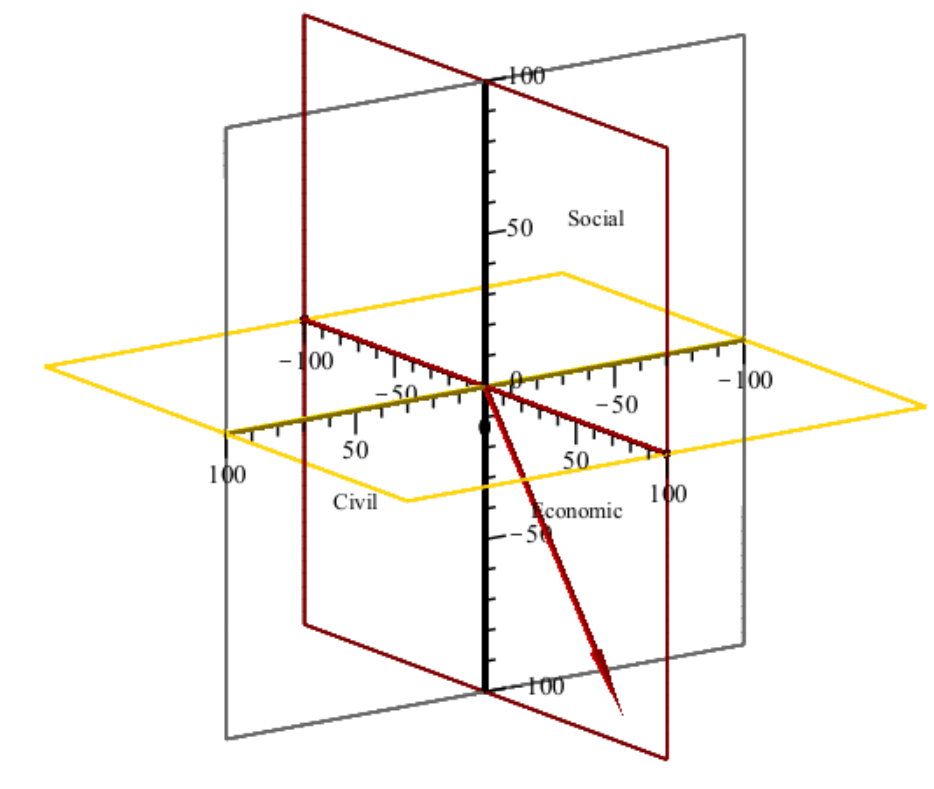
\includegraphics[width=0.6\textwidth]{vectorA}
\caption{\footnotesize An example of a Political Entity represented as a vector}
\label{exVector}
\end{figure}

\qquad If we add another Political Entity $\bm{B} = 24\civ - 9\econ - 38\soc$ we can now find the norm between them by first finding the difference vector $\bm{B} - \bm{A} = (24 - (- 12))\civ + (-9 - 59)\econ + (-38 - (- 97))\soc = 36\civ - 68\econ + 59\soc$. Then, it is possible to find the magnitude (length) of a vector by finding the square root of the sum of the squares of the components of the vector. So $|\bm{B} - \bm{A}| = \sqrt{36^2 + (-68)^2 + 59^2} = 96.96$. So the norm of $\bm{A} \tand \bm{B}$ is 96.96 (you'll notice in Figure \ref{exNorm} that this is very similar to the Pythagorean Theorem). This norm between two Political Entities is used in almost all interactions that take place in the model. For example, when the Preference List for each Voter is being determined, the Candidates are sorted in order of their norm with the Voter, with the shortest norm first. Then, any Candidates whose norm with the Voter is larger that the Voter's Approval Radius is removed from the list. This leaves each Voter with a list of the Candidates inside their Approval Radius, in order of how close they are.
\begin{figure}[H]
\centering
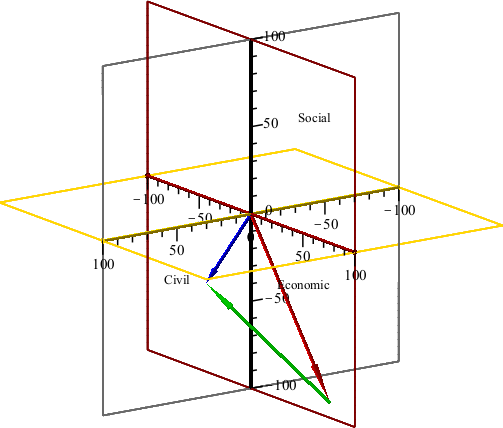
\includegraphics[width=0.6\textwidth]{vectorABC}
\caption{\footnotesize An example of the difference vector used to find the norm between two Political Entities}
\label{exNorm}
\end{figure}

\qquad A very similar process is used to assign Citizens to Parties. For each Citizen, the list of Parties is sorted in descending order by their norm with the Citizen, then the closest Party is checked to make sure its norm with the Citizen is less than or equal to the Citizen's Approval Radius. After this, different things happen depending on if the Citizen is a Voter or a Candidate. If the Citizen is a Voter and the Party is within the radius, then the Voter is assigned that Party; if it is not in the Radius, the Voter simply does not have a Party. If the Citizen is a Candidate and the Party is within the Candidate's Approval Radius, then that Candidate is assigned that Party and is added to the Party's internal Candidate list. If the norm of the Party and Candidate is greater than the Candidate's Approval Radius, then a new virtual Party is created with the same position as the Candidate. This is an independent Party. If any independent Party ends up with enough funding to keep running a Candidate, then the independent Party with the most Funding becomes a persistent virtual Party while the others are removed from the simulation. Unaffiliated Citizens will have the chance to join it before the next election. \\

\qquad While the norm between two Political Entities is a very important quantity, it is not used directly in all of the model's operations. A Party's Funding is determined by the percentage of the total Voters that are aligned to the Party, as well as the percentage of (first choice) votes received by the Party's Candidates. Again, this process is not analogous to real world fundraising, but it is suitable for this model. After an election, the Party and the top choice Candidate on the Preference List of each Voter is checked and counted. For each whole percentage of total Voters (who voted for at least one Candidate) affiliated with a Party, that Party gains 1 unit of funding, while for each whole percentage of total first choice votes for a Party's Candidates, that Party gains 5 units of funding. Each Candidate requires at least 27 units of funding in order to run (these specific numbers where chosen to provide a reasonable amount of progression after each iteration). \\

\qquad If, at the end of an election, a Party does not have enough funding to run all of their Candidates, the Party goes through a dropping process. During dropping, total Funding is divided by 27\footnote{This value is semi-arbitrary; it does not specifically represent anything, but was chosen to produce more desirable results.} (the amount needed to run a single Candidate) and rounded down to an integer, which will be the maximum number of Candidates the Party can afford. The Party's Candidates are then sorted in order of votes received, and the lowest performing Candidates are then dropped so that the Party now has the maximum number of Candidates it can afford to run. When a Candidate is dropped, it is removed from the Party's Candidate List and the Candidate's party affiliation is removed. \\

\qquad Next, the Voting System goes through its own dropping process. First, we find all the Candidates that were dropped from their Party in the previous step by checking the Party of each Candidate. If a Candidate does not have a Party, then a persistent virtual Voter is created with the same position as the Candidate, and then the Candidate is removed from the simulation. This part of the process is analogous to a politician deciding to no longer run. Next, all of the Independent Parties are sorted in order of Funding. The Independent Party with the most Funding, provided it is enough to run at least one Candidate, is transitioned into a non-Independent Party and becomes persistent, and any Candidates left in the other Independent Parties are dropped from their Party (though not from the simulation). Lastly, the amount of Candidates each Party has is checked. Any Party that does not have any Candidates are removed from the simulation, which would be any Party that did not have enough Funding to run a single Candidate and all but (possibly) the best performing Independent Party. \\

\qquad Nudging, and Satisfaction along with it, also use the norm for their function, but in a different way than voting and assigning Parties. Each Voter's Satisfaction value is determined on a weighted scale based on their norm with the winning Candidate. Since the axes range from -100 to 100, the largest the norm between two Political Entities can be is $\sqrt{(100 - (- 100))^2 + (100 - (- 100))^2 + (100 - (- 100))^2} = 346.41$. This would be one Political Entity at the very corner of the coordinate system, and the other Political Entity at the opposite corner. The lowest a norm between two Political Entities could be is 0, if both Political Entities have the exact same position. From these two extreme cases, we can take $\frac{346.41}{2} = 173.21$ to be the midpoint between political agreement and disagreement in our coordinate system. To find a Voter's Satisfaction, we first subtract their norm with the winner from this midpoint to find a kind of ``agreement score." Then we take a random number from a Gaussian distribution with standard deviation of 10 centered at the value of the agreement score to be that Voter's Satisfaction value. The winner's Performance is found in a similar way, although the norm is not used. The winner's Performance is based on the winner's Representation Score. Since a score of 50\% is the midpoint of possible Representation Score values, the winner's Representation Score is subtracted by 50 to get the ``balanced representation score." A random number from a Gaussian distribution centered at the value of the balanced representation score with a standard deviation of 10 is then set as the winner's Performance Value. Since more popular Candidates are more likely to have a high Performance score, and in reality a voter is more likely to be satisfied with the performance of a popular representative, the winner's Performance value is added to each Voter's Satisfaction value. This makes the maximum Satisfaction value within one standard deviation on both of the Gaussian distributions equal to 243.21, with the minimum value within one standard deviation on both distributions equal to -243.21. \\

\qquad After Satisfaction values have been determined, Voters are nudged. The nudging process also uses the norm, but in a very different way from the rest of the model, and a full explanation requires further discussion of vectors and their properties. A vector can be thought of as having two fundamental properties: a direction and a magnitude. There is a special kind of vector that has a magnitude of exactly 1, called a ``unit vector." Because a unit vector has a magnitude of 1, there is a sense in which they are purely directional. By dividing any vector by its own magnitude, we can create a unit vector that has the direction of the original vector, so by dividing the difference vector between two Political Entities by their norm (so long as their norm is not equal to zero), can get the unit in the direction from one Political Entity directly to the other; we'll label this unit difference vector as $\vhat{d}$. By doing this for every Voter with the winner, we get the direction from each Voter directly to the winner, as seen in Figure \ref{exUnitVectors} (if the norm is zero, we avoid dividing by zero by simply setting $\vhat{d} = 0\civ + 0\econ + 0\soc$).
\begin{figure}[H]
\centering
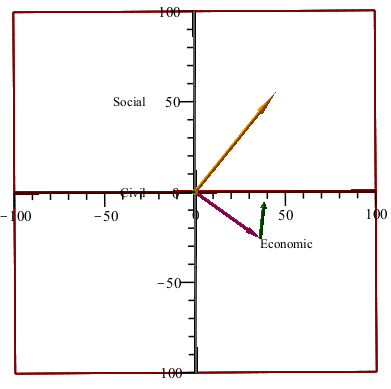
\includegraphics[width=0.6\textwidth]{dhatnudge}
\caption{\footnotesize The unit vector pointing from a Voter to the winning Candidate}
\label{exUnitVectors}
\end{figure}

\qquad For the actual nudging, Voters with a Satisfaction value above 80 or below -80 (i.e. in the top/bottom third of possible values within one standard deviation on both distributions) are moved in the direction of $\vhat{d}$ an amount equal to 25\% of the Voter's Satisfaction value. Since Voters with low satisfaction have negative Satisfaction values and vise-versa for high satisfaction, this will cause highly satisfied Voters to be nudged toward the winner (an example of this can be seen in Figure \ref{exNudge}), highly dissatisfied Voters to be nudged away from the winner, and neutral Voters to stay put. If a Voter would be nudged past a value of -100 or 100 (i.e. past the bounds of the coordinate system), they are instead nudged just to the edge. For example, say a Voter that has Civil component with absolute value $\left|C\right| \le 100$ would be nudged to have a new Civil component with absolute value $\left|C^\star\right| > 100$. That Voter would instead be nudged to $100 \times \frac{C^\star}{\left|C^\star\right|}$. This way, if $C^\star$ is less than -100, $\frac{C^\star}{\left|C^\star\right|} = -1$ so the new value of $C$ will be -100; and if $C^\star > 100$, then $\frac{C^\star}{\left|C^\star\right|} = 1$ so the new value of $C$ will be 100. This method is used for each axis to make sure all Political Entities say within the boundaries of the coordinate system.
\begin{figure}[H]
\centering
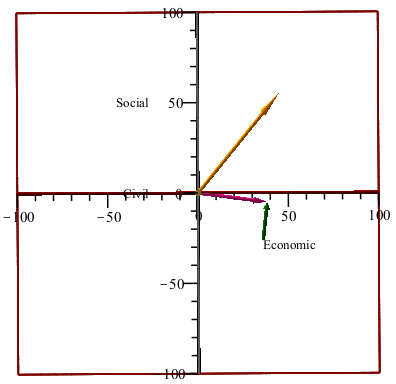
\includegraphics[width=0.6\textwidth]{nudged}
\caption{\footnotesize An example of a Voter being nudged toward the winner}
\label{exNudge}
\end{figure}

\qquad This mechanism models a kind of incentive for candidates to try and win with as much support as possible, since a popular representative is more likely to be reelected. If a Candidate wins an election with a very low number of votes, Voters are very likely to move away from that Candidate and, in turn, closer to other Candidates that could then become the next winner. While this behaviour \textit{is} a very important dynamic to model, nudging also plays a different, arguably more important role in the simulation: the avoidance of steady states. In applied Mathematics, a steady state is a set of inputs to a system such that the output is exactly equal to the input. What this looks like for our model is that a set of Voters, Candidates, and Parties is fed into the Voting System, and after the election there is no change to this set; no Candidates are dropped from their Party, no Parties are dropped from the simulation. It should be clear to see that without nudging, this occurs once all independent Parties have either been dropped or become persistent, and all Parties end an election with enough funding for all of their Candidates. For most random sets of initial conditions, that happens after only the second or third election. With non-randomized nudging (i.e. if the nudging process did not include any random values and was instead determined entirely by norms and votes), a steady state only occurs when all independent Parties have either been dropped or become persistent, all Parties end an election with enough funding for all of their Candidates, \textit{and} all Voters either have a Satisfaction value between -80 and 80 or have been nudged all the way to the edge of the coordinate system. Clearly, this is a much rarer occurrence, and in most cases it takes many more elections to reach a steady state than without any nudging. \\

\qquad Another way nudging helps avoid steady states is that stable equilibria are rare. A stable equilibrium is a steady state of a system where a small perturbation from the steady state quickly goes back to the steady state. For example a ball in the center of a large bowl is at a stable equilibrium; if you push it a bit in any direction, the ball just rolls back to the bottom of the bowl. An unstable equilibrium, on the other hand, is a steady state where a small perturbation causes the system to veer far from that steady state. This would be like if the ball was instead balanced on the top of an upside-down bowl; any small push will cause the ball to roll all the way off. Looking at nudging in our model, a very dissatisfied Voter moves away from the winner, so if that Candidate is reelected, the Voter will be even less satisfied and move even farther away. The opposite will happen for a very satisfied Voter, they move toward the winner and if that Candidate is reelected they move even closer. Because of this any state of the system that is very close to a steady state will tend to move away from it. This is helped even more by the introduction of randomness into the process. Even if the simulation has reached a steady state, there is still the possibility that a Voter's Satisfaction value of the winner's Performance value will randomly end up many standard deviations away from the mean, pushing the system back into motion. \\

%0000000000000000000000000000000000000000000000000000000000000000000000000000000000
%0000000000000000000000000000000000000000000000000000000000000000000000000000000000
\section{Limitations} \label{Limitations}
%0000000000000000000000000000000000000000000000000000000000000000000000000000000000
%0000000000000000000000000000000000000000000000000000000000000000000000000000000000
\qquad When simulating any complex system, simplifications must be made in order for the model to be feasibly implemented. It would be totally impractical, and maybe impossible, to model all the opinions, interactions, systems, and environmental factors that go into a specific voter's choice of political preferences; and such a model may not even be desirable if it could be made. In many ways, the quality of a simulation is based on a balance of accuracy of results verses the computational resources needed to get those results; a perfect simulation that takes eight years to process does no one any good. What you want is as simple a model as you can make for your desired level of accuracy, and so simplifications are made. However, every simplification and assumption added to a model brings with it new limitations for what your model can say about a system. For this project, most of these limitations unsurprisingly stem from the central assumption of our model: that political preference and voting behaviour can be represented within a Cartesian coordinate system. \\

\qquad Some ambiguity comes from the fact that each axis in the coordinate system has opposing concepts at their ends, so there are two independent interpretations of what a specific placement on the axis means. In the first interpretation, each axis can be thought of as a spectrum from one concept to another, like a sliding scale where someone placed at the origin ($\bm{O} = 0\civ + 0\econ + 0\soc$) would have no preference either way on any issue. Alternatively, specific placement can be the average of many different positions, so that someone at the origin could have very strong opinions on most or all issues, but all their positions average out to the center. This is an inherent limitation of the compass system. However, we are using this system to understand how a specific voter is going to vote. A voter at the origin is going to behave the same way regardless of whether they are an `averages to zero' voter or a `center of the slider' voter. This argument extends to any position in the coordinate system; which ever interpretation is used, the expected voting behaviour does not change. Additionally, while the possibility space (the set of all possible values something can have) of what political ideals a voter can hold is very different between the two interpretations, the possibility space of where voters are placed on in the coordinate system is actually the same. Since both the behaviour of an voter and the possible placements of voters is identical between the two possible interpretations, we can treat them as being equivalent, meaning this nuance can safely be ignored. \\

\qquad This fact, that we are interested only in the modeling of voting habits, allows for another important simplification. In reality, an individual voter may hold strong opinions on all axes, but think that one issue is more important than the others, and therefore vote differently than this model would predict. This problem could be solved by adding individualized weighting to each issue, however that would break the visual correlation between a Voter's position in the coordinate system and their voting preference. This would be exemplified as a voter with a position $\bm{V} = 100\civ + 100\econ + 100\soc$ but who believes that Civil policies are supremely important above all else; that voter would appear to vote as if their position was actually $\bm{V}^\star = 100\civ + 0\econ + 0\soc$. Since this is supposed to be a demonstrative tool, that correlation is important. Because of this, we assume that a Political Entity's placement is already reflective of their individual weighting of the issues. This way the weighting of each axis can be treated as equal when determining votes, preserving the visual correlation between preference and voting. \\

\qquad Other limitations stem from different kinds of tie conditions that can be encountered. The most obvious type of a tie is when more than one Candidate has the highest number of votes: an `election-level tie.' For this kind of tie, a tie breaking procedure is included in the model that chips away at some of our assumptions. Firstly, in most real world elections, an exact tie is essentially impossible. Despite this, most voting systems do have a procedure to deal with ties, and the most common way to resolve a tie is a runoff election. This is a completely new round of voting, except that the only Candidates that were part of the tie are in the running. An additional wrinkle comes from an assumption we made about Candidates. Up to this point, we have assumed in this model that the number of Voters so totally eclipses the number of Candidates that the votes from Candidates are negligible. However, in the case of an election-level tie we see that these votes may not actually be negligible. To remedy this, all Candidates that were not part of the tie are replaced by virtual Voters with the same position. These virtual Voters only exist for this runoff vote. This is the first step in our tie breaking procedure, and it is usually sufficient to break the tie. There is, however, the distinct possibility that the runoff will also result in a tie. If the runoff vote had more that two Candidates, we can simply have another round of runoff voting, but if a runoff between only two Candidates still results in a tie, more must be done to determine a winner. \\

\qquad In the case of a two way tie after runoffs, we need to temporarily discard one other assumption made in the model, namely the assumption that initial conditions on the simulation are a complete description of the political landscape. As mentioned, an election-level tie is essentially unheard of in real world elections, and this is because of the monumental scale of a nation-state. This model, however, often is operating at a fraction of that scale. We take advantage of this fact to break the tie. By taking our list of Voters to be a representative sample of the population, rather than the population itself, we can introduce a new virtual Voter at the average position of all Voters. By finding which of the tied Candidates this average Voter prefers, we can extrapolate that if the election had been run with a full population instead of a sample more Voters would prefer that Candidate over the other. Thus, the tie is broken by finding the average Civil, Economic, and Social components of all Voters, then creating a virtual Voter at that average position with an Approval Radius large enough to ensure both Candidates are within it, and finally giving one more vote to the Candidate that is closer to the virtual average Voter. \\

\qquad The other kind of tie that is encountered is a `vote-level tie.' This occurs whenever a Voter cannot distinguish their preference between two candidates; they are exactly as preferable as each other. For our model this happens whenever more than one Candidate is exactly the same distance from a specific Voter. In a real election, this would not be an issue, the voter would simply choose one to rank higher arbitrarily. However, for our model there is no way to simulate this arbitrary choice in a way that is both unbiased \textit{and} deterministic. Recall that while the overall model is lightly stochastic, we require that every individual election be fully determined by its initial conditions. We could randomly assign one Candidate to be ranked higher, sacrificing the election's determinism; or we could axiomatically designate some other factor to by the decider, biasing the simulation towards that factor. In order to solve this problem, we must again temporarily abandon one of our assumptions, this time the assumption that a Voter's voting preference is decided only by their norm with a Candidate. Looking again to the real world, an individual voter very often associates much more strongly with a Party than any particular candidate (ANES). Taking advantage of this, in the case of a vote-level tie, we can compare the two Candidates' norms to the Voter's Party. If the Voter does not have a Party, we can use a virtual Voter in the same position with an Approval Radius of 400 to find the Party that is closest to the Voter and compare the Candidates' norms to that Party. This is enough to resolve almost all ambiguities, however it is still possible for the tie to persist in this situation if the Candidates are both the same distance from the Voter's Party. At this point we can turn to the Candidate's Parties, and compare their norms with the Voter. But, even that is not enough though, as with the correct symmetries (illustrated in Figure \ref{tieSymmetry}) this can still result in a vote-level tie. Under normal circumstances, the likelihood of this situation occurring is miniscule, however, because there are curtain vote-level ties that this model cannot resolve, we are simply forced to limit the allowed states of the system to exclude these situations.
\begin{figure}[H]
\centering
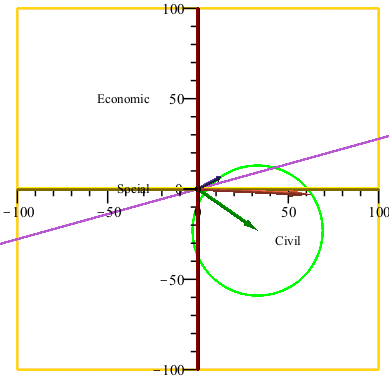
\includegraphics[width=0.6\textwidth]{vectorGcircleline}
\caption{\footnotesize The symmetry needed for an indisambiguable vote-level tie (Voter is green, circle shows dNorm with red and blue Candidates, purple line shows where the Party can be positioned to cause the catastrophic tie)}
\label{tieSymmetry}
\end{figure}

\qquad The final limitations that require discussion are related to identical Political Entities. Simply put, there is no problem with caused by two Voters being identical; the program can run perfectly well even if all the Voters are identical. There are, however, issues with identical Candidates and Parties. In principle, the model should work with identical Candidates. In practice though, having two or more Candidates with the exact same position makes is much more likely to have a catastrophic vote-level tie, so Candidates are not allowed to have the exact same position. This is achieved by forcing newly created Candidates to have a norm that is greater than 0 with all other Candidates; if any of their norms are 0, that Candidate is removed a replaced with a new random Candidate. Similar problems also occur if Parties are allowed to be identical, so they are also subject to the norm $>$ 0 restriction. The last issue stemming from identical Political Entities happens when a Voter has identical position to a Candidate, specifically to a winning Candidate. If a Voter has identical position to a winner, than during nudging, since their norm is 0, $\vhat{d}$ would have non-real number components. However, as has already been discussed earlier, a simple solution is to check for this possibility when nudging and to reset $\vhat{d}$ if it occurs. \\

%0000000000000000000000000000000000000000000000000000000000000000000000000000000000
%0000000000000000000000000000000000000000000000000000000000000000000000000000000000
\section{Examples} \label{Examples}
%0000000000000000000000000000000000000000000000000000000000000000000000000000000000
%0000000000000000000000000000000000000000000000000000000000000000000000000000000000

\qquad A set of example experiments using the tool have been generated to be used as a reference. This section will not show program output, because the output is currently still in development. Instead, the results of the elections are presented as charts. These examples all used the same pool of 200 Voters and 5 Candidates. For simplicity, it was assumed that every Candidate had a different Party, so to accomplish this only one Party was generated, and it was far off the coordinates system so that no Citizens would align with it, instead the only Parties were the Independent Parties tied to each Candidate. To improve the clarity and demonstrative value, the pool of Voters was manually curated so that none abstained from voting completely. One sample election of each type was run using these initial conditions.\\

For First Past the Post, Candidate B earned the most votes and is elected as the winner.

\begin{figure}[H]
\centering
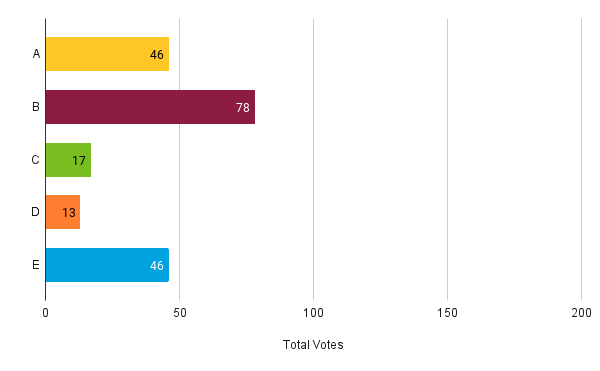
\includegraphics[width=0.8\textwidth]{Firstchart}
\end{figure}

For Approval, Candidate E earned the most votes, so the winner is different. Here is one of the clearest examples of a how changing voting system can improve our democracy. Instead of the winner representing less than half of the Voters, the winner of this election was voted for by over 75\% of voters. As you will see in the following examples, First Past the Post, the most commonly used voting system in real elections, (usually) produces the least representative winners.

\begin{figure}[H]
\centering
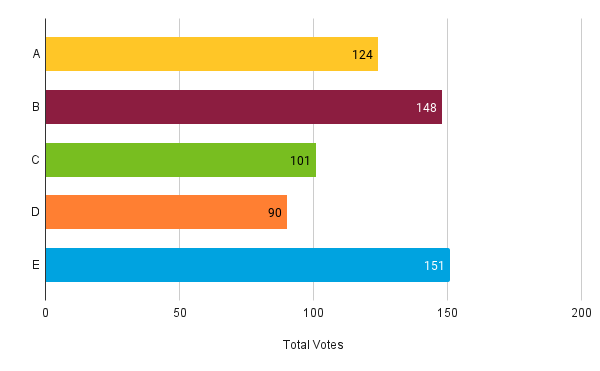
\includegraphics[width=0.8\textwidth]{Appchart}
\end{figure}

\qquad Since First Past the Post is only first choice votes, the first stages of the two ranked choice systems are exactly the same as the First Past the Post election. In our case, no Candidate has received more than 100 votes (100 being 50\% the number of ballots cast) so we move on to step two.\\

For Bucklin, we add second choice votes to each Candidate's total. Below, those second choice votes are color coded based on that Voter's first choice. After adding second choice votes, both Candidate B and Candidate E have more that 100 votes, but Candidate E has the most, so they are the winner.

\begin{figure}[H]
\centering
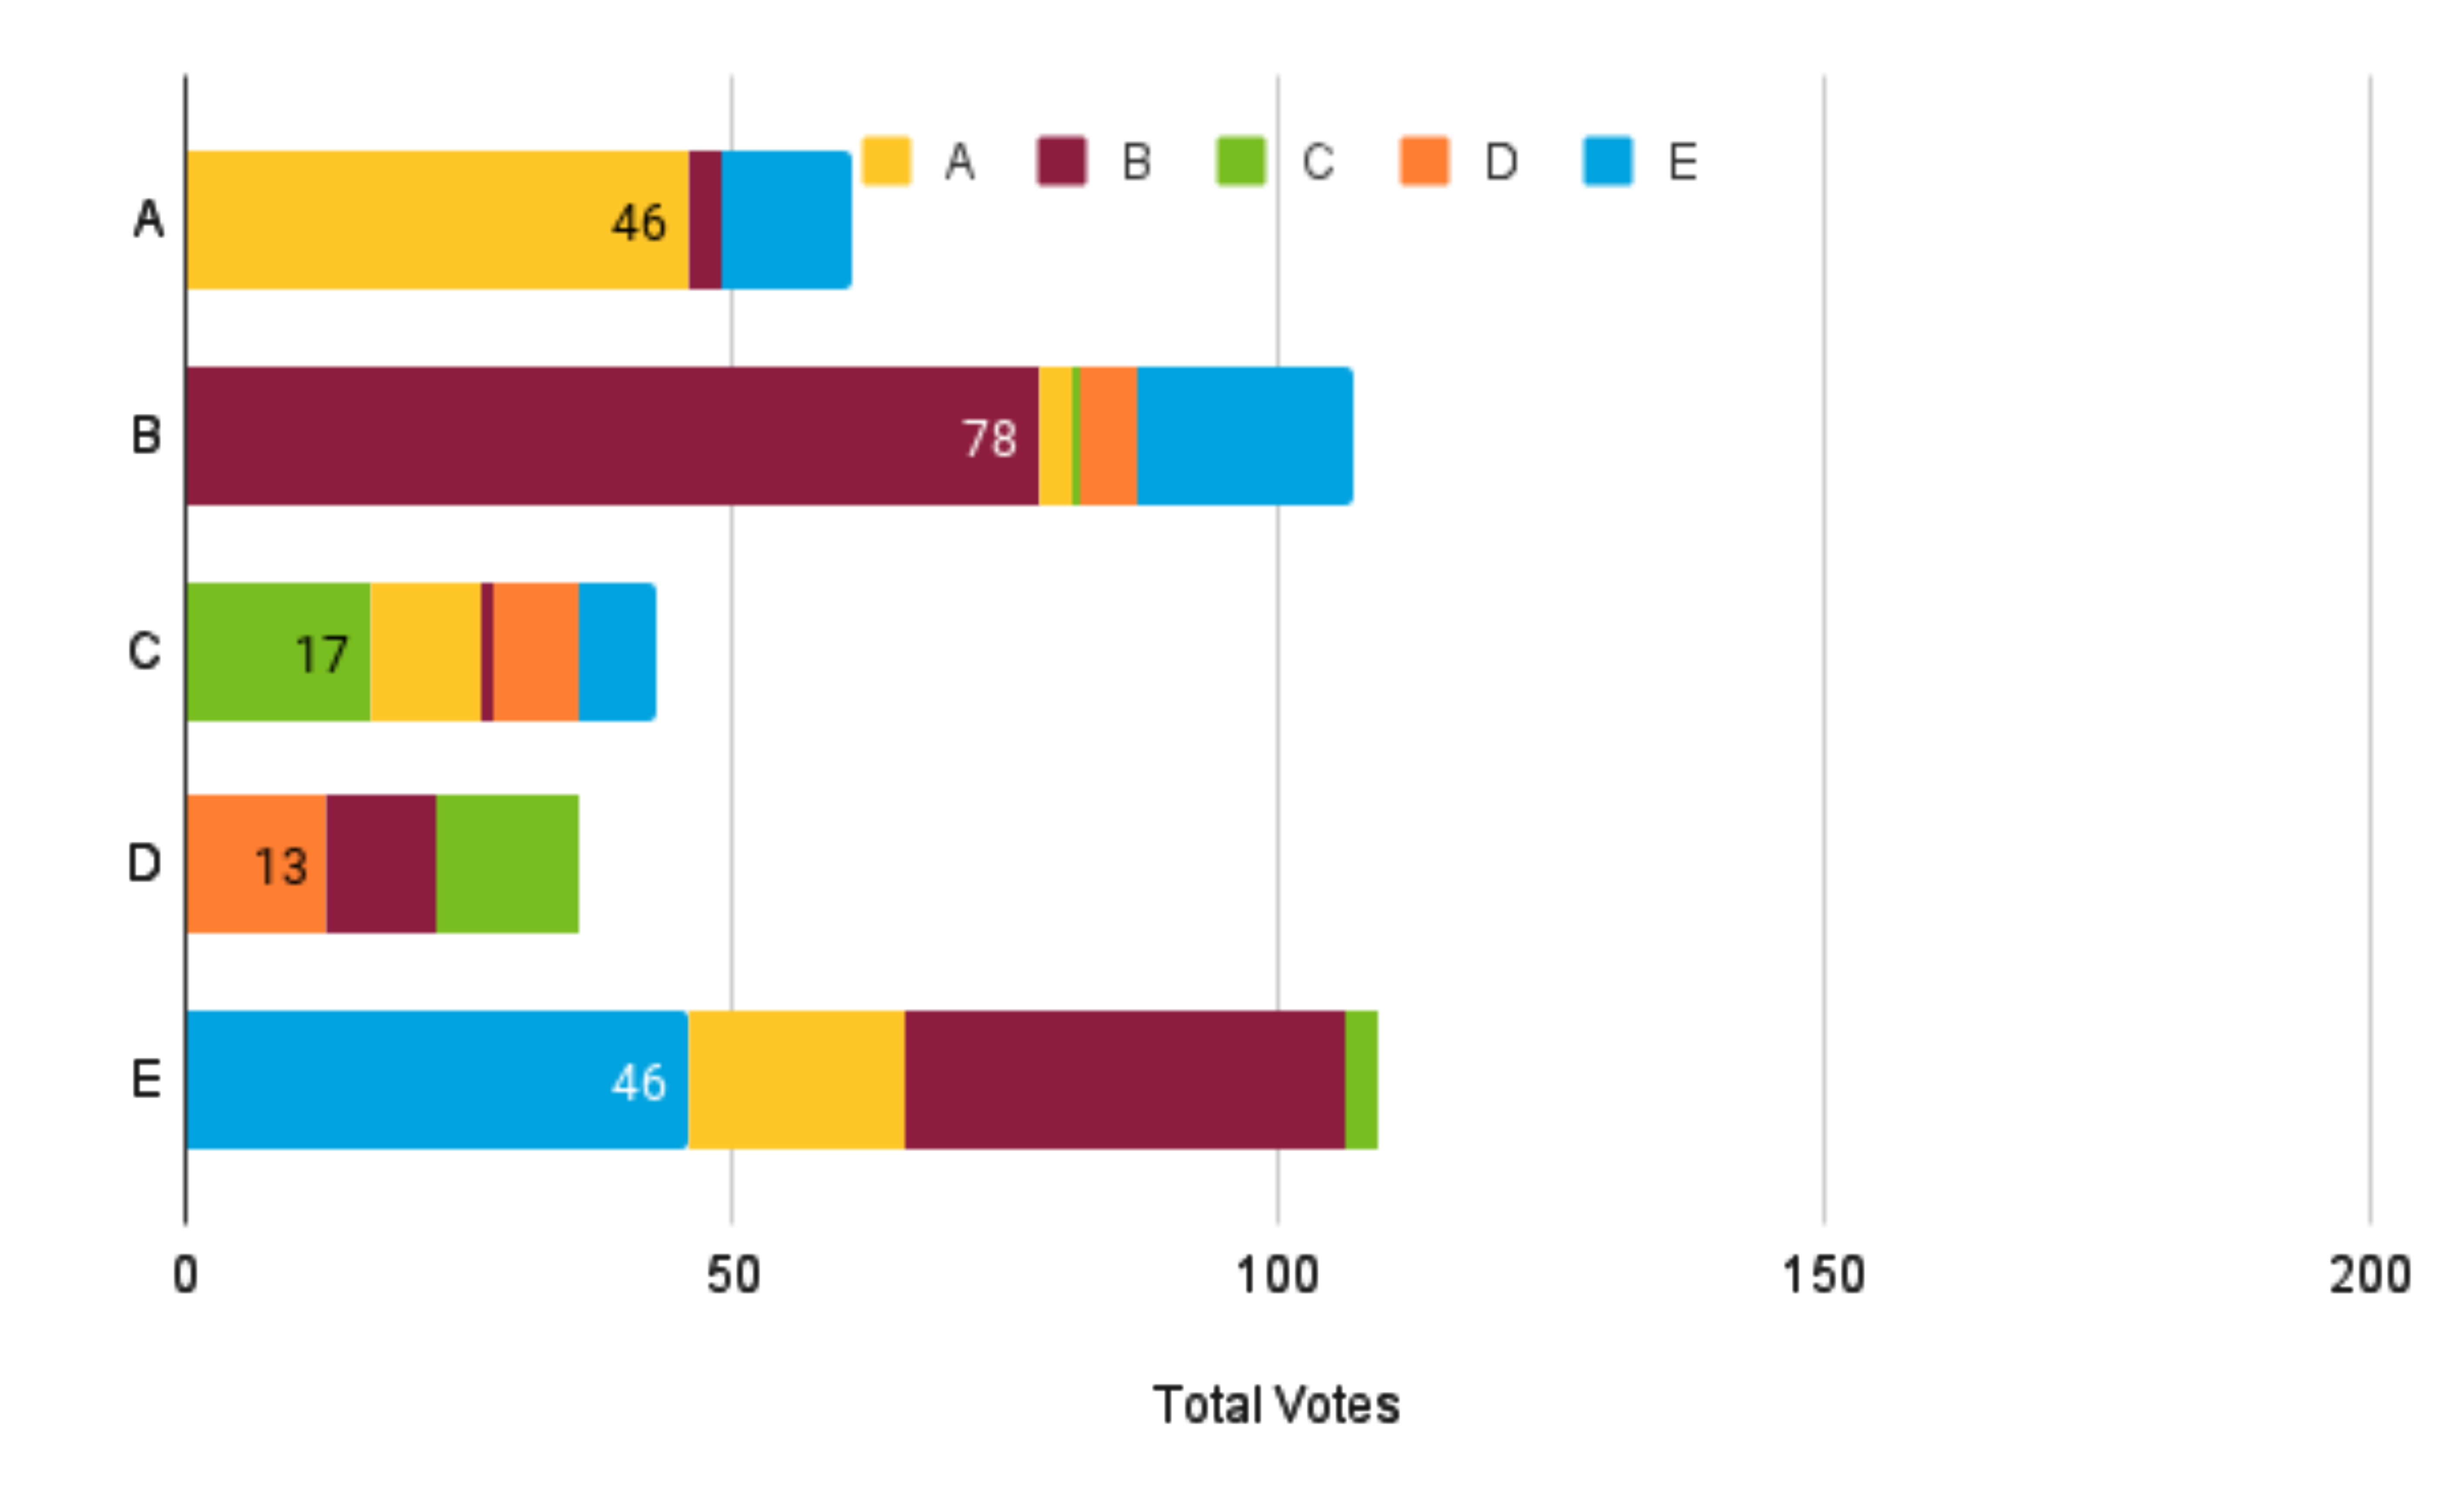
\includegraphics[width=0.8\textwidth]{Buckover}
\end{figure}
\begin{figure}[H]
\centering
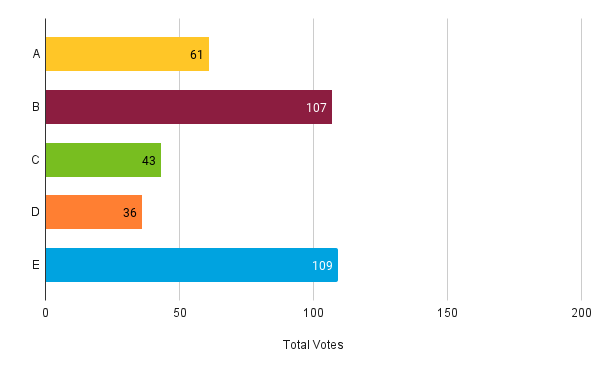
\includegraphics[width=0.8\textwidth]{Buckchart}
\end{figure}

For Instant Runoff, Candidate D had the least votes, so they are removed and those votes go to the second choices. After adding those votes, all Candidates still have less than 100 votes. Candidate C now has the lowest number of votes, so they are removed and the votes are given to the next choices. Now Candidate E has the fewest votes, so those votes are given to next choices. After adding these votes, Candidate B now has more that 100 votes, so they are the winner. 

\begin{figure}[H]
\centering
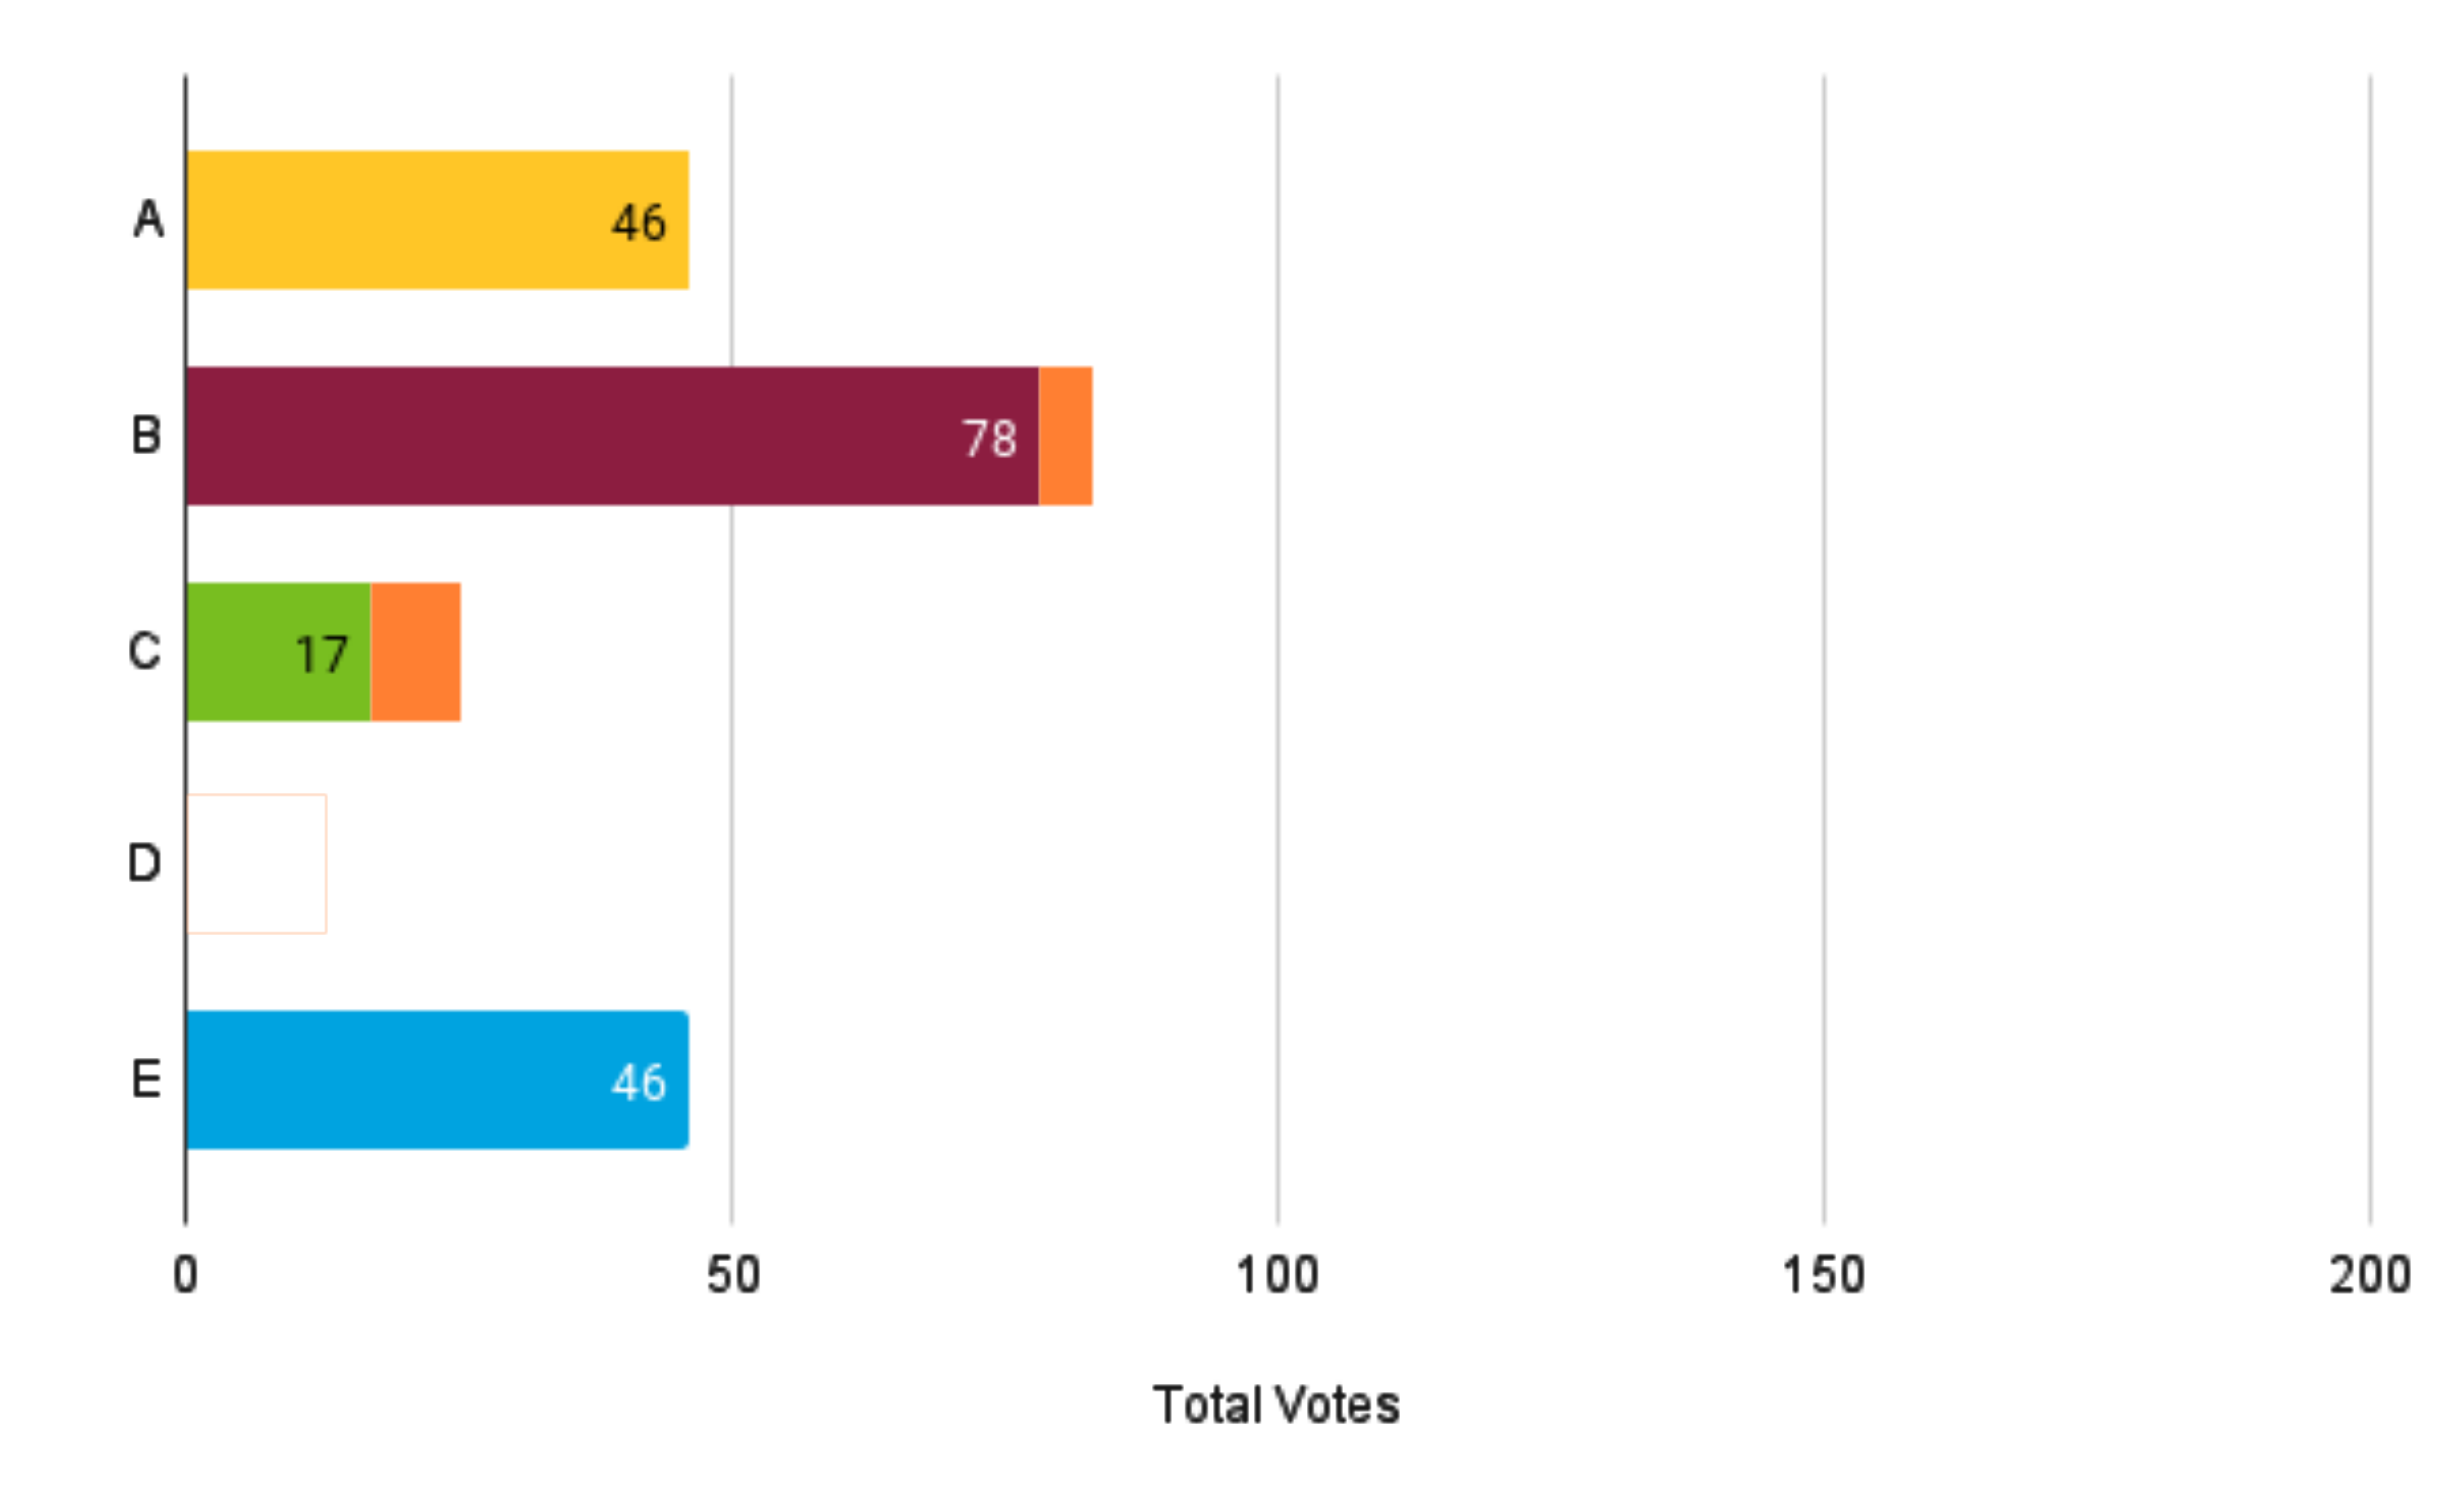
\includegraphics[width=0.8\textwidth]{Altover1}
\end{figure}
\begin{figure}[H]
\centering
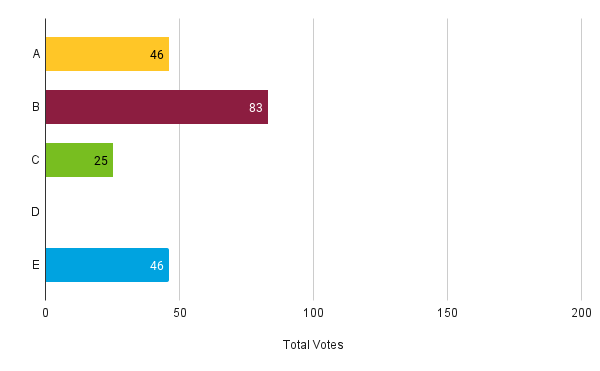
\includegraphics[width=0.8\textwidth]{Altchart1}
\end{figure}
\begin{figure}[H]
\centering
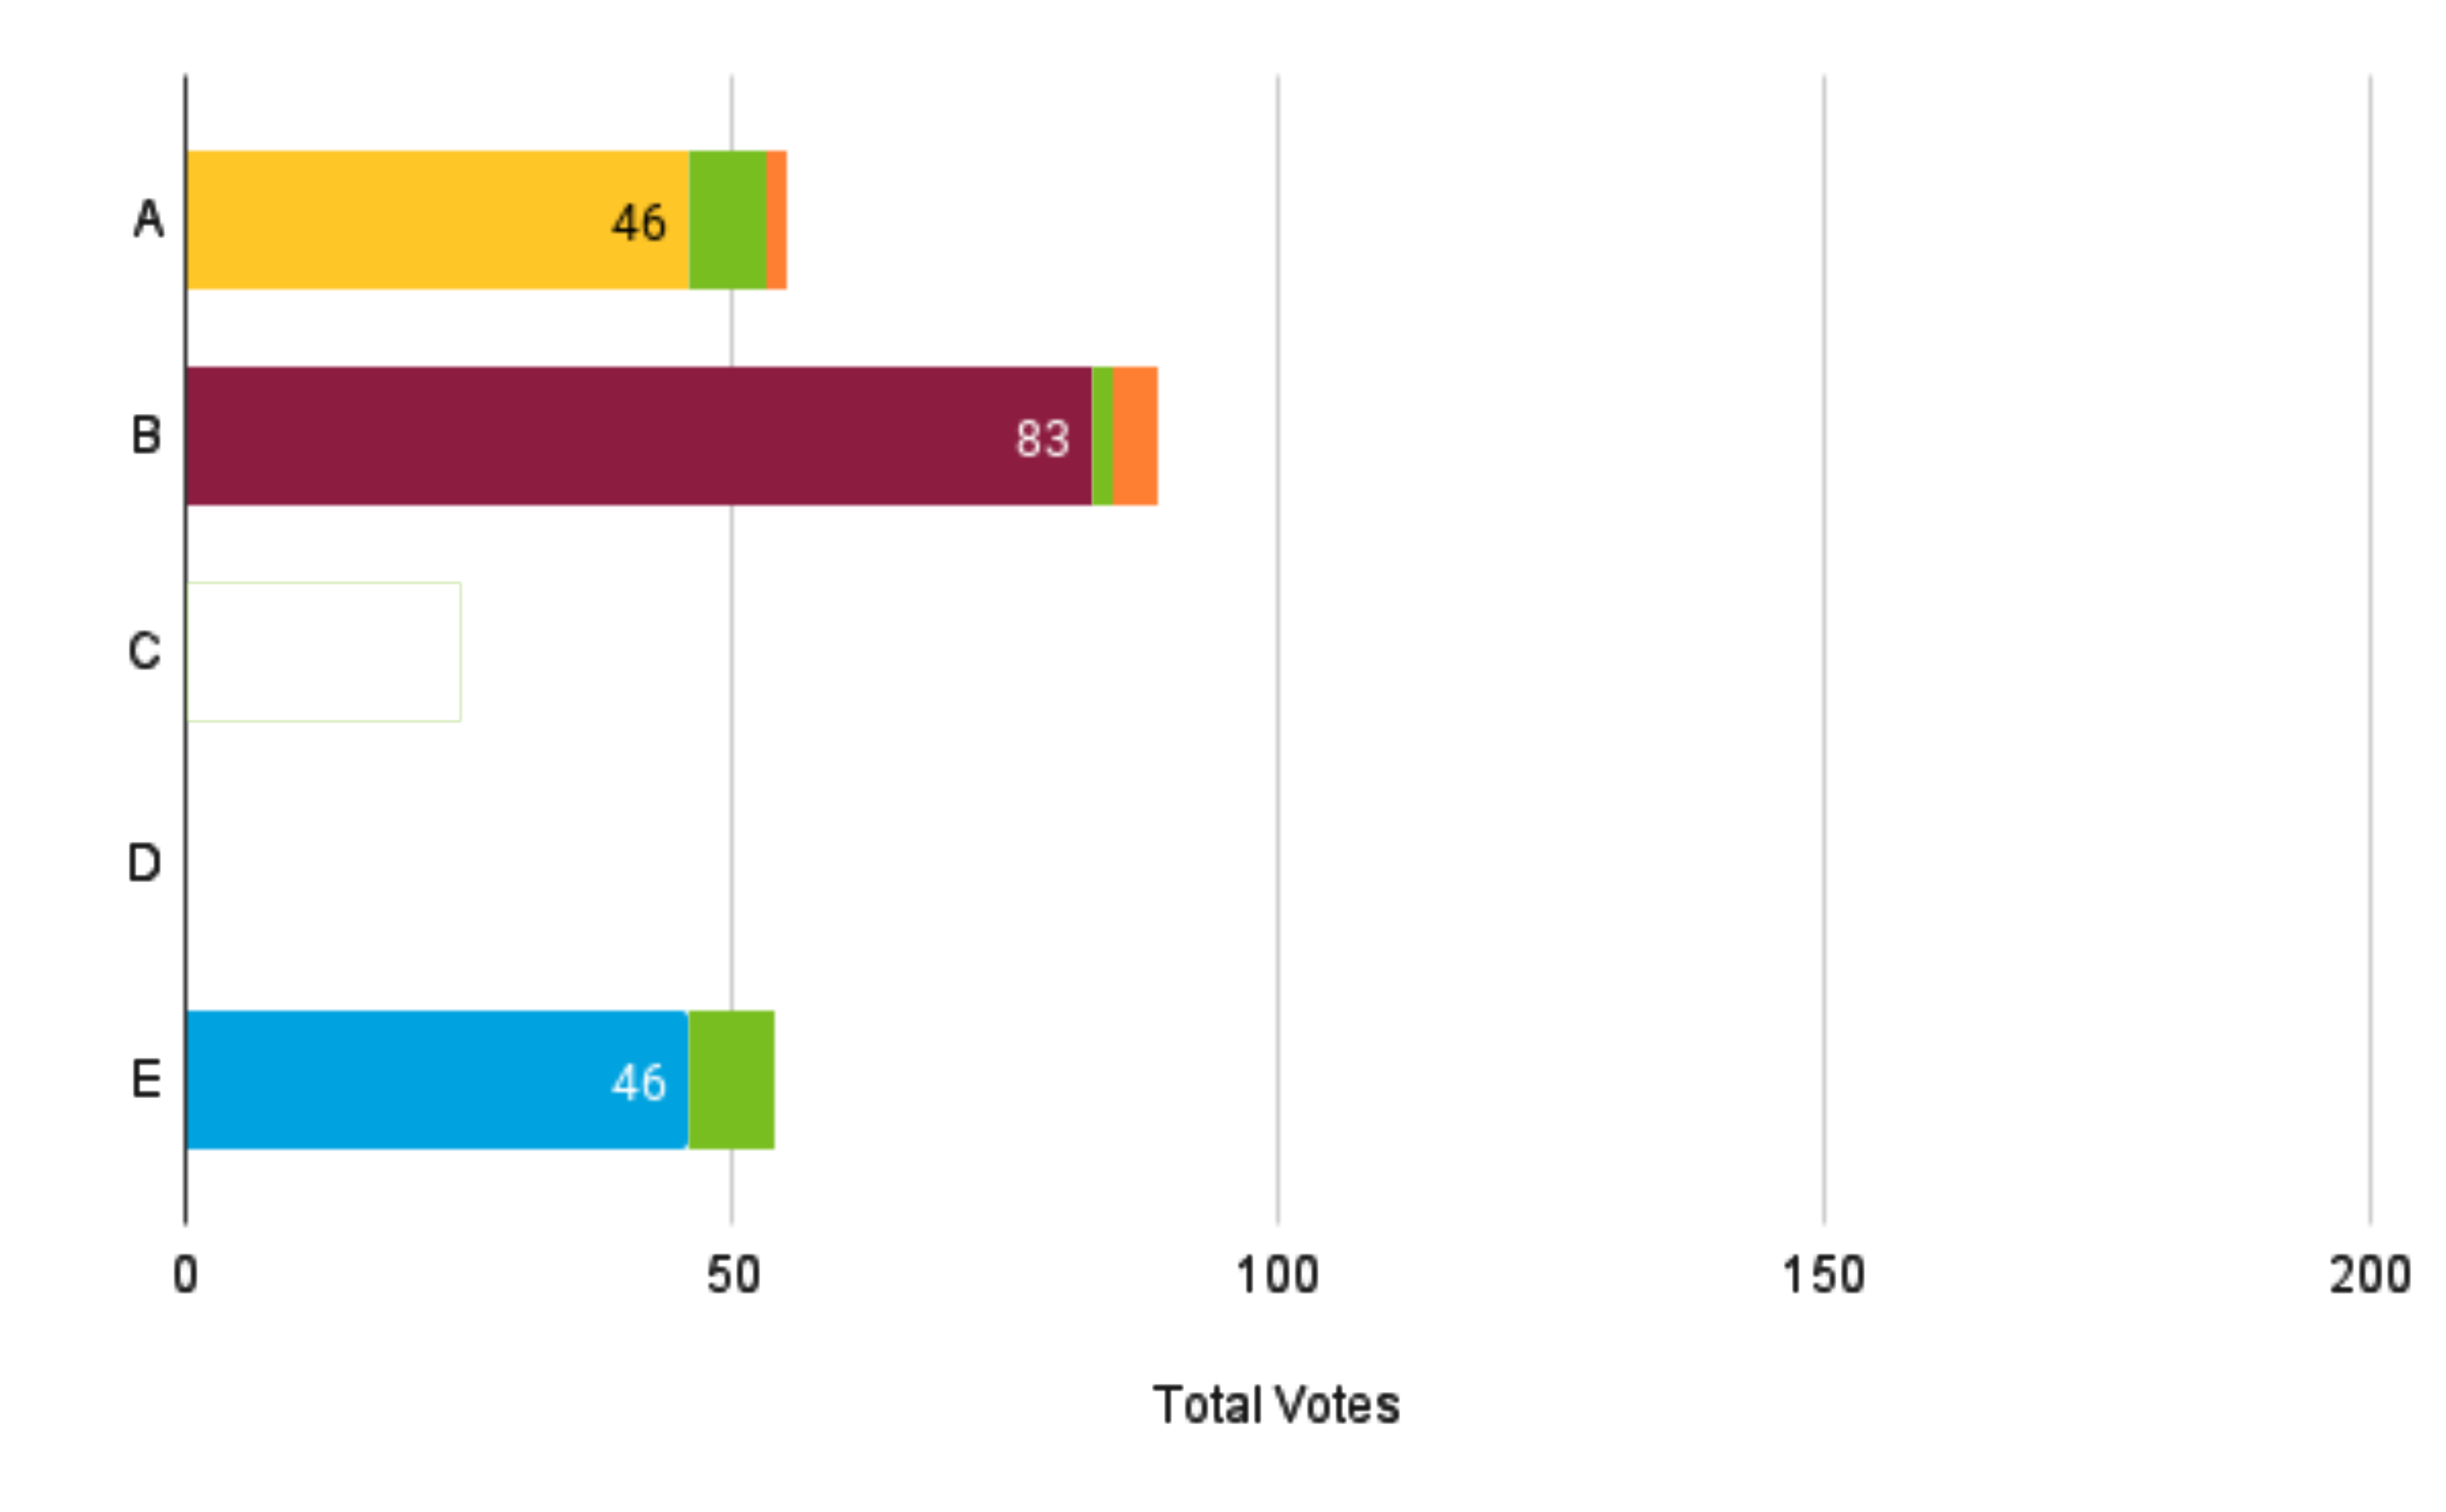
\includegraphics[width=0.8\textwidth]{Altover2}
\end{figure}
\begin{figure}[H]
\centering
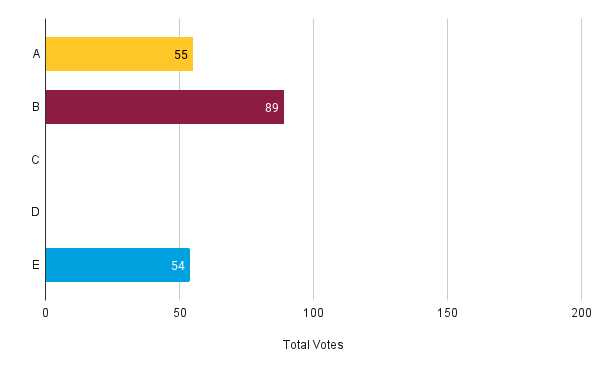
\includegraphics[width=0.8\textwidth]{Altchart2}
\end{figure}
\begin{figure}[H]
\centering
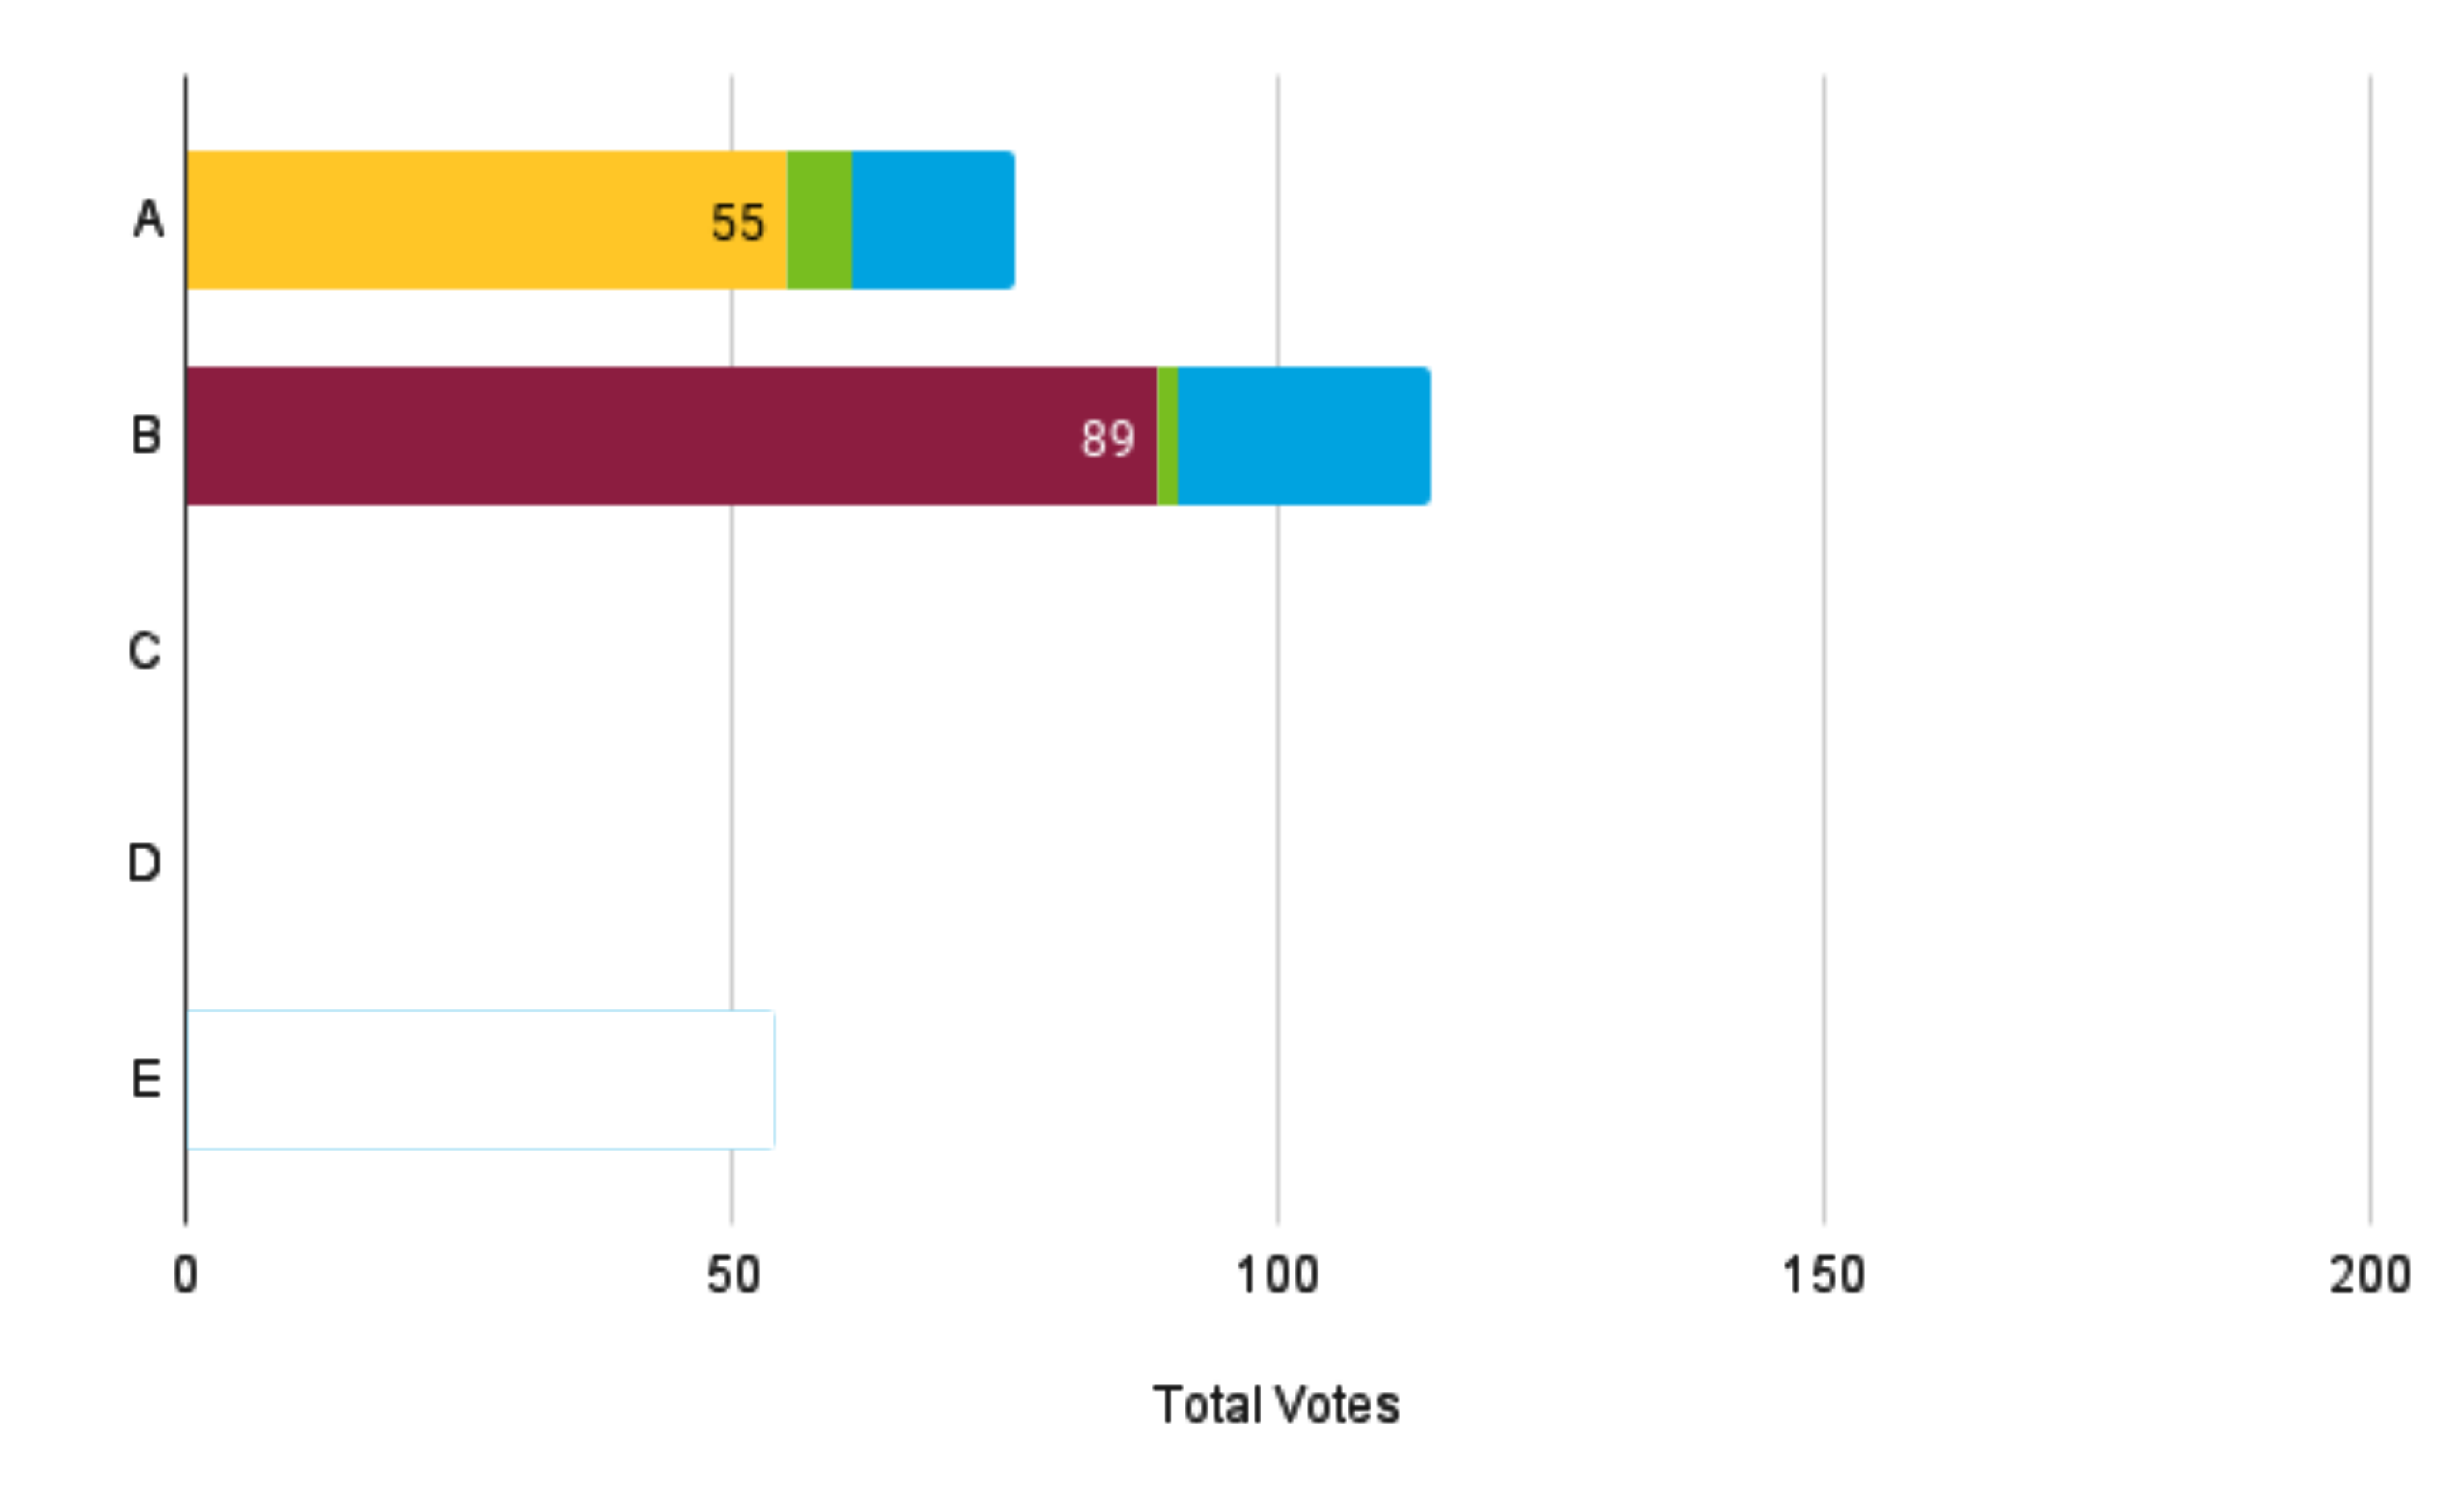
\includegraphics[width=0.8\textwidth]{Altover3}
\end{figure}
\begin{figure}[H]
\centering
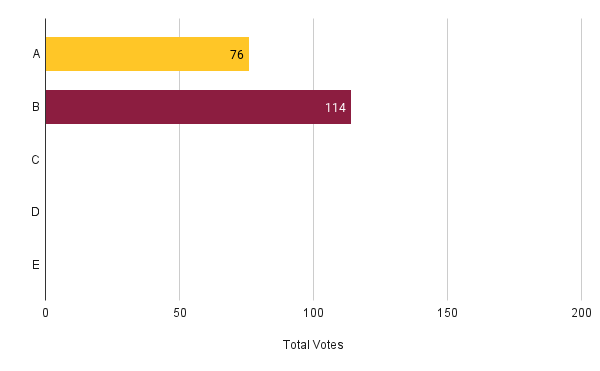
\includegraphics[width=0.8\textwidth]{Altchart3}
\end{figure}

\qquad One of each kind of Fairness Measure was run for each election. First Past the Post was the only to fail the Representation Score, but this is slightly misleading. Normally, if enough Voters abstain or do not specify enough later preferences, all of these Voting Systems can fail this criterion; in these examples the Voter pool was curated to maximum turnout, which inflated the Representation Score. For the Condorcet Test, First Past the Post had all Candidates in the Smith set, and Instant Runoff had A, B, and E in the Smith set so they passed. Approval and Bucklin Voting both elected Candidate E, but E lost to B pairwise, so they failed. For Independence of Alternatives, Bucklin Voting passed, but all the rest failed to a clone of the winner. For Later no Help/Harm, First Past the Post and Instant Runoff passed, with Approval and Bucklin both failing since E Voters specifying more later preferences caused Candidate B to win.

%0000000000000000000000000000000000000000000000000000000000000000000000000000000000
%0000000000000000000000000000000000000000000000000000000000000000000000000000000000
\newpage
\section{Appendix A: UML Class Diagrams} \label{AppA}
%0000000000000000000000000000000000000000000000000000000000000000000000000000000000
%0000000000000000000000000000000000000000000000000000000000000000000000000000000000

The following UML class diagrams capture the voting system design using astah, a tool for developing and software specifications (see \cite{astah}).

\begin{centering}
\begin{figure}[H]
\centering
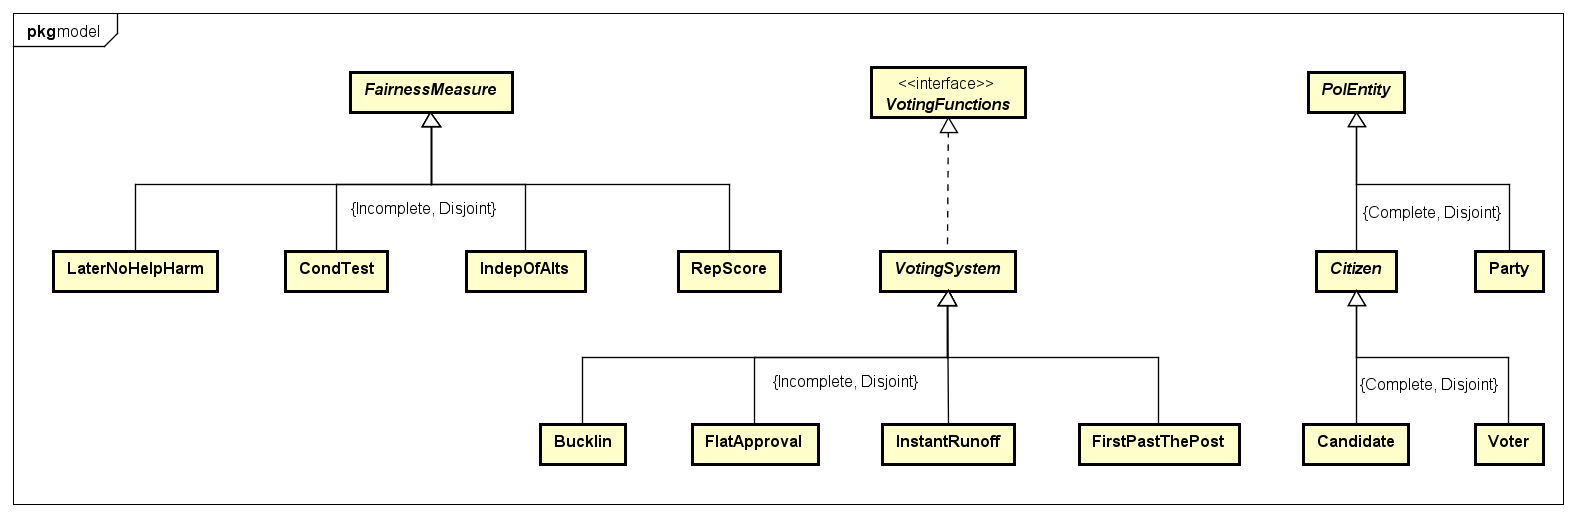
\includegraphics[width=1.2\textwidth, angle=90]{SimpleUML}
\end{figure}
\footnotesize Simple version of the full UML Diagram

\begin{figure}[H]
\centering
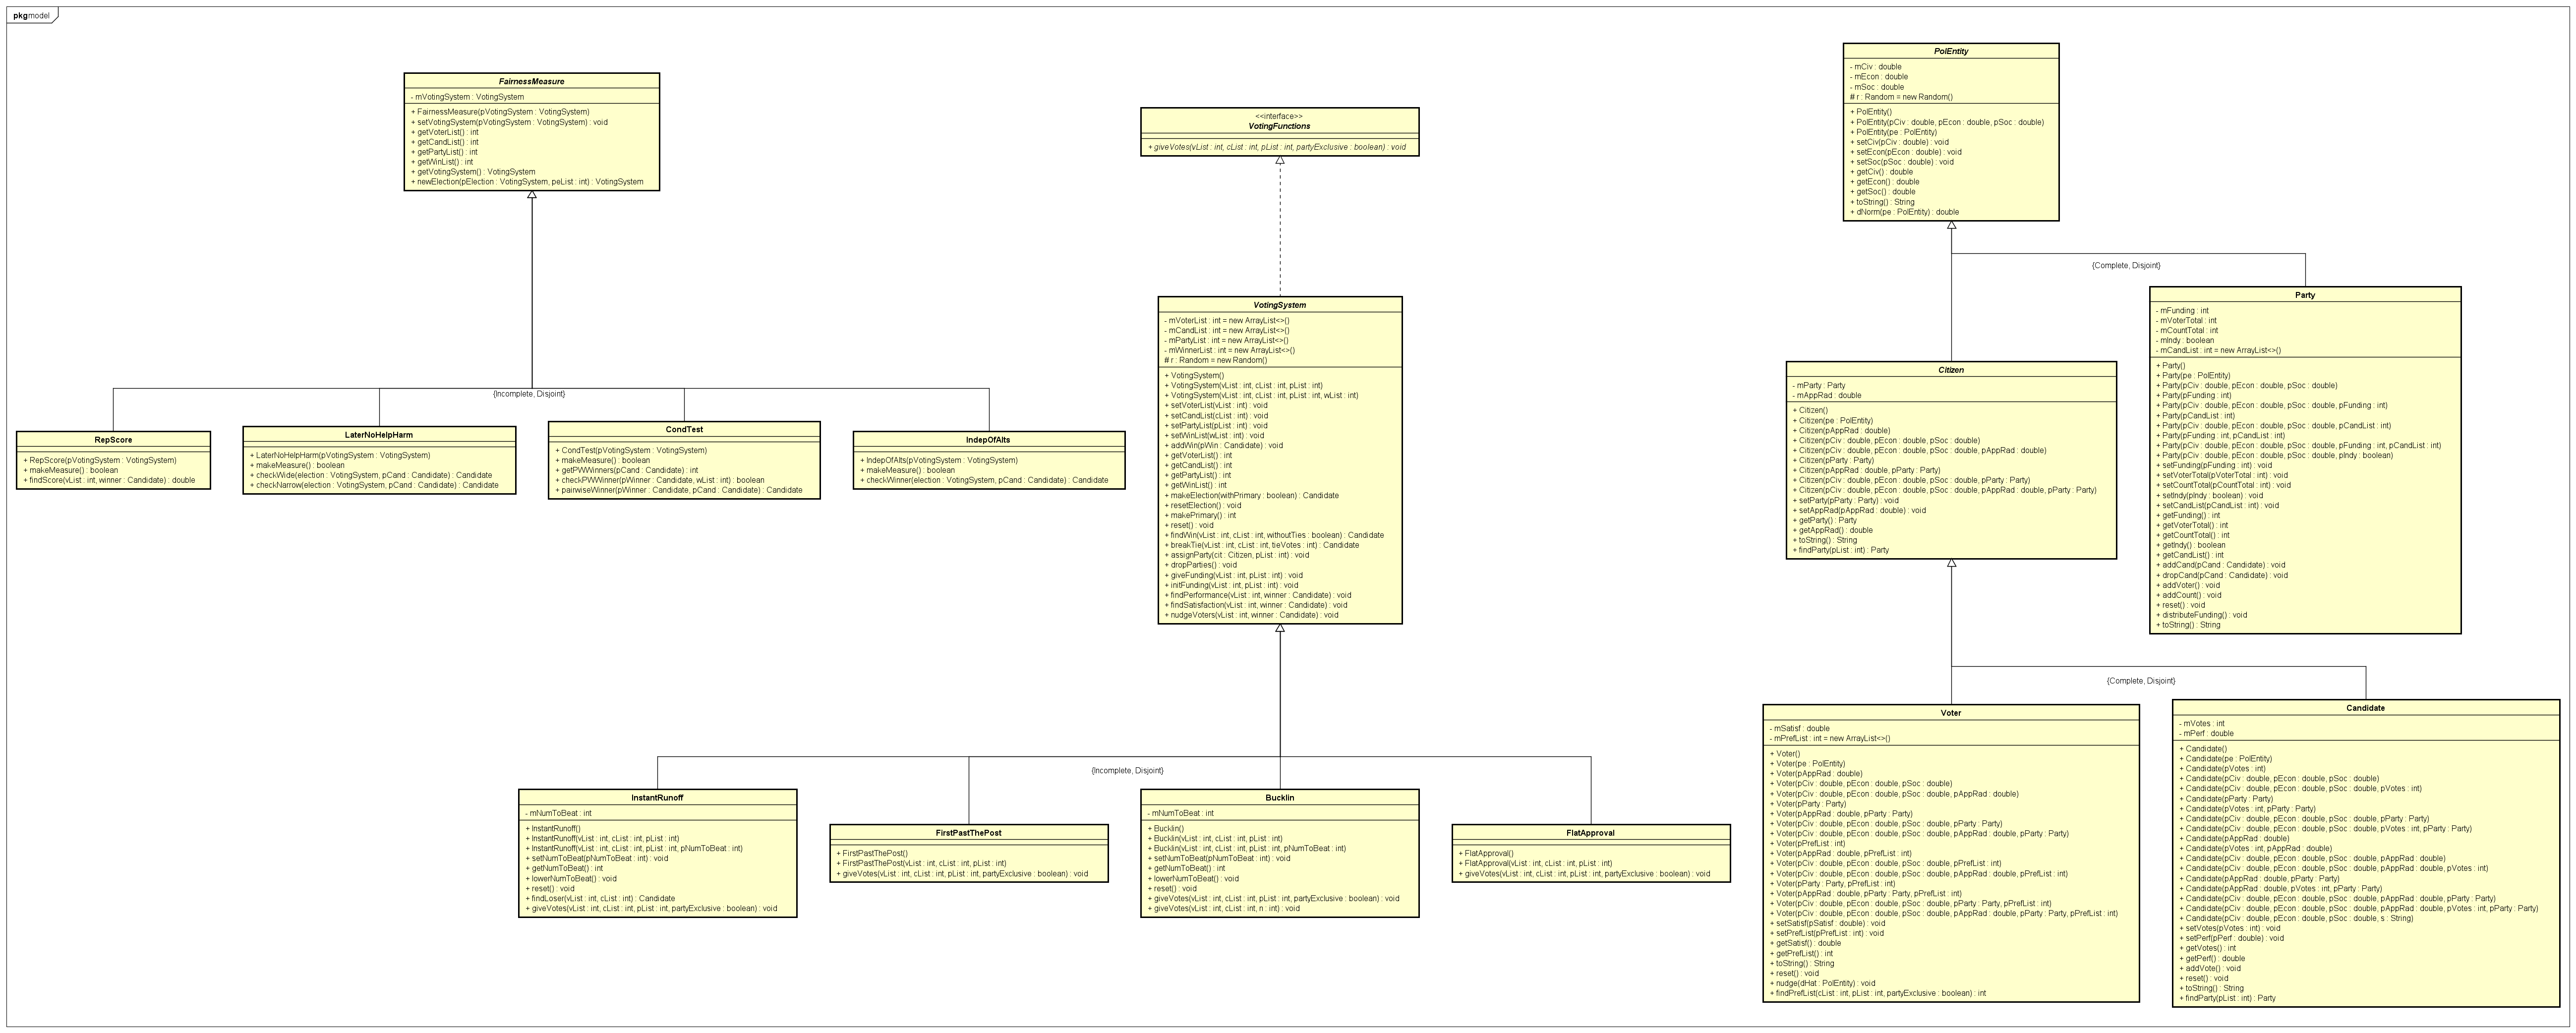
\includegraphics[width=1.3\textwidth, angle=90]{DetailedUML}
\end{figure}
Detailed version of the full UML Diagram (zooming in may be helpful

\begin{figure}[H]
\centering
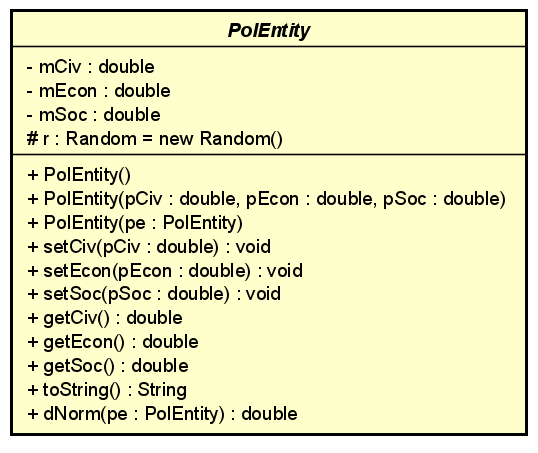
\includegraphics[width=0.7\textwidth]{PolEntity}
\end{figure}

\begin{figure}[H]
\centering
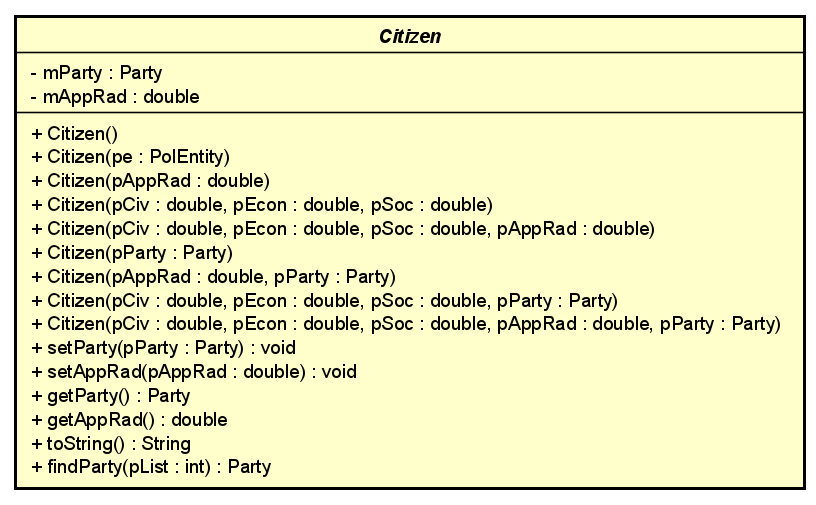
\includegraphics[width=0.7\textwidth]{Citizen}
\end{figure}

\begin{figure}[H]
\centering
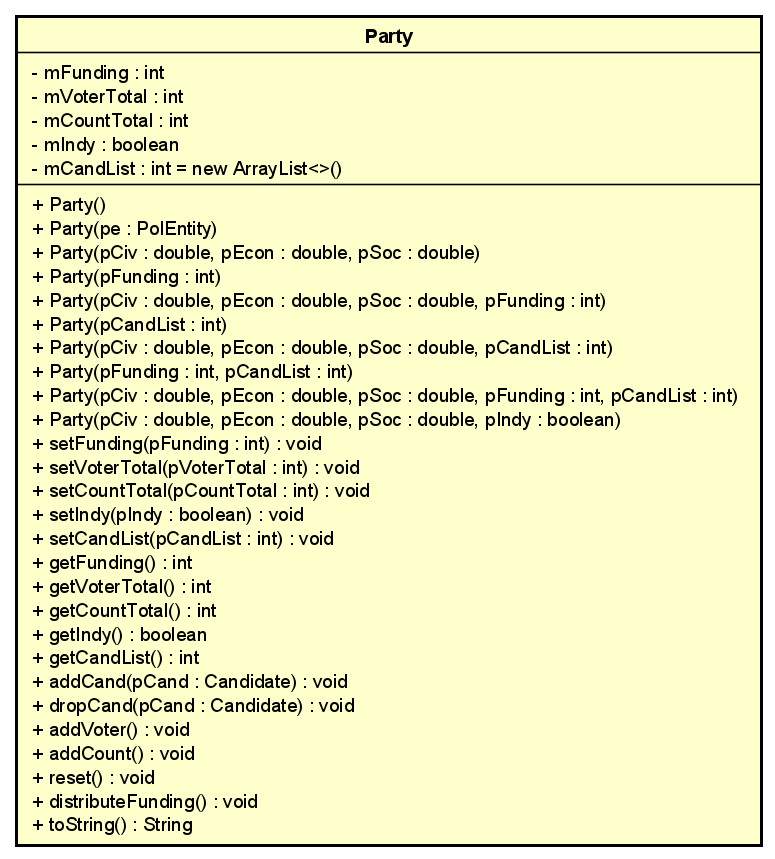
\includegraphics[width=0.7\textwidth]{Party}
\end{figure}

\begin{figure}[H]
\centering
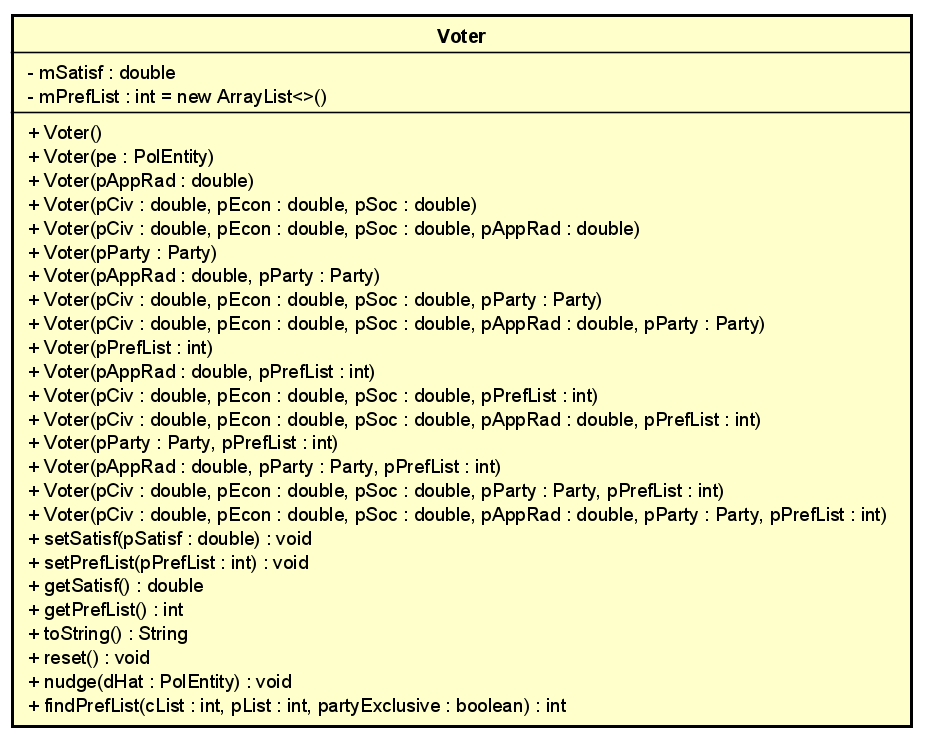
\includegraphics[width=0.7\textwidth]{Voter}
\end{figure}

\begin{figure}[H]
\centering
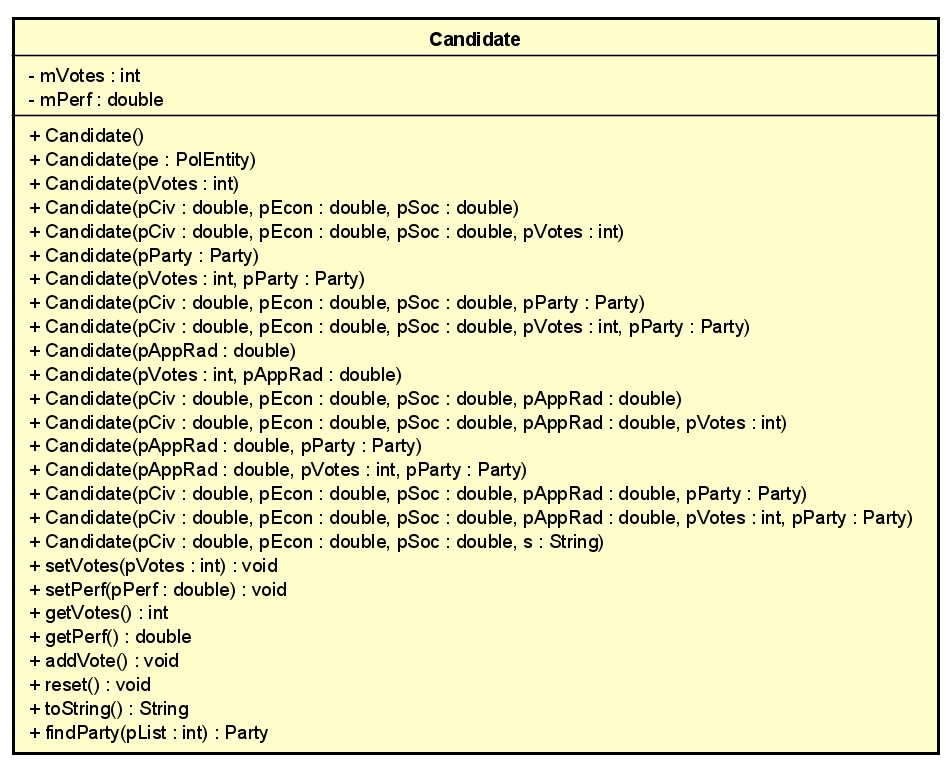
\includegraphics[width=0.7\textwidth]{Candidate}
\end{figure}

\begin{figure}[H]
\centering
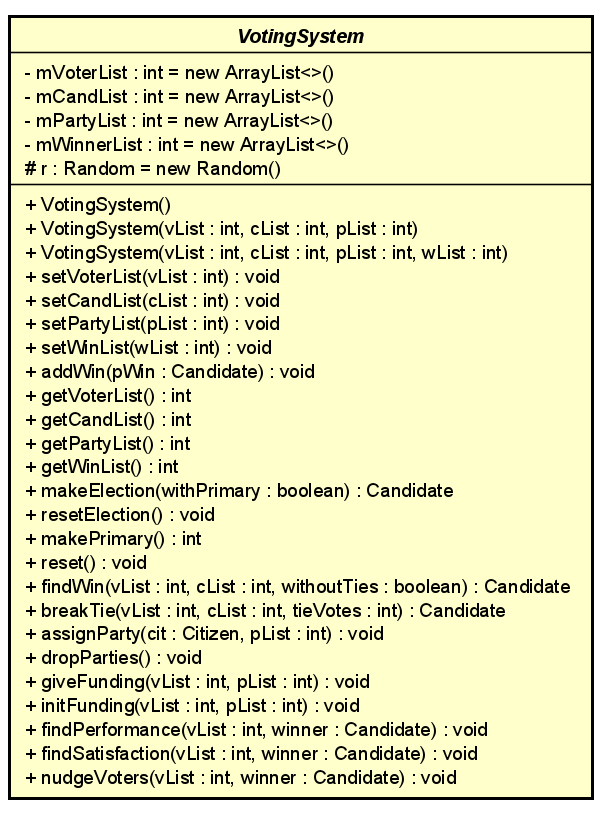
\includegraphics[width=0.7\textwidth]{VotingSystem}
\end{figure}

\begin{figure}[H]
\centering
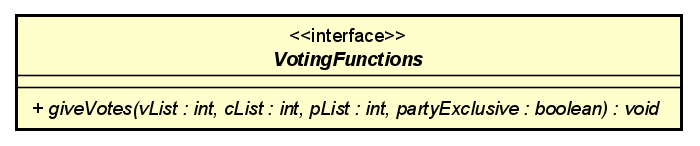
\includegraphics[width=0.7\textwidth]{VotingFunctions}
\end{figure}

\begin{figure}[H]
\centering
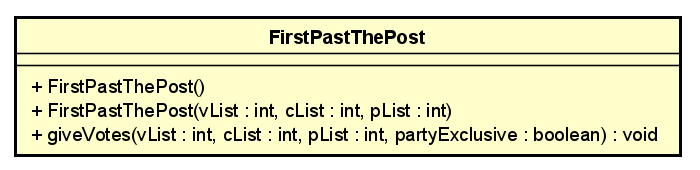
\includegraphics[width=0.7\textwidth]{FirstPastThePost}
\end{figure}

\begin{figure}[H]
\centering
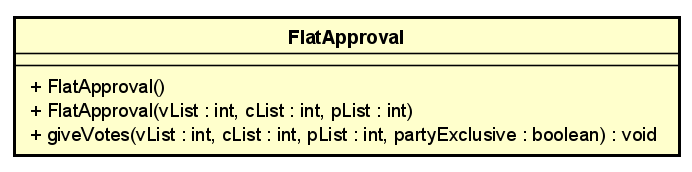
\includegraphics[width=0.7\textwidth]{FlatApproval}
\end{figure}

\begin{figure}[H]
\centering
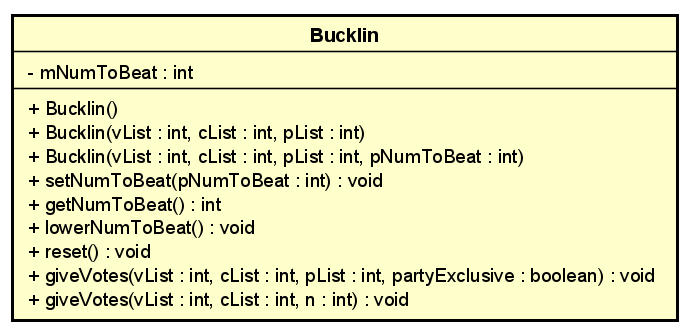
\includegraphics[width=0.7\textwidth]{Bucklin}
\end{figure}

\begin{figure}[H]
\centering
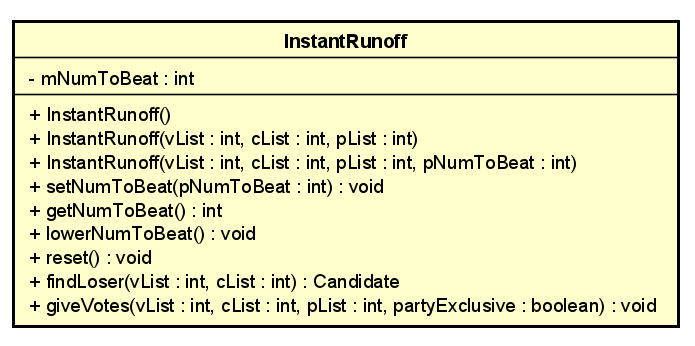
\includegraphics[width=0.7\textwidth]{InstantRunoff}
\end{figure}

\begin{figure}[H]
\centering
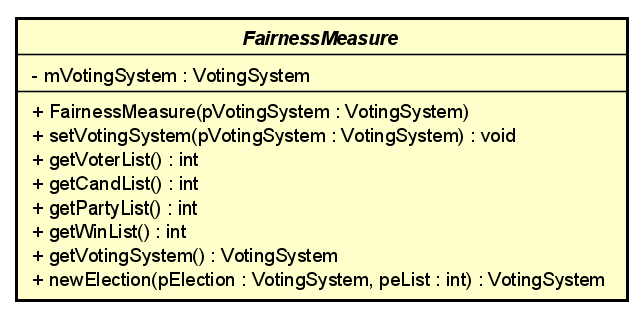
\includegraphics[width=0.7\textwidth]{FairnessMeasure}
\end{figure}

\begin{figure}[H]
\centering
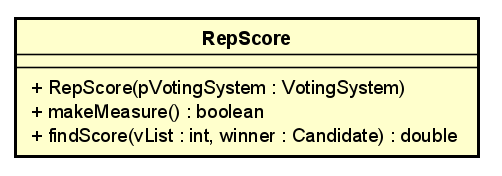
\includegraphics[width=0.7\textwidth]{RepScore}
\end{figure}

\begin{figure}[H]
\centering
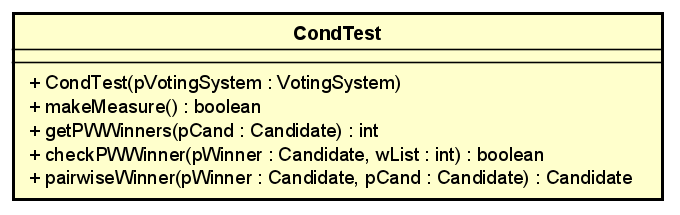
\includegraphics[width=0.7\textwidth]{CondTest}
\end{figure}

\begin{figure}[H]
\centering
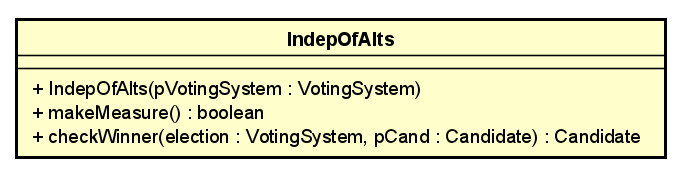
\includegraphics[width=0.7\textwidth]{IndepOfAlts}
\end{figure}

\begin{figure}[H]
\centering
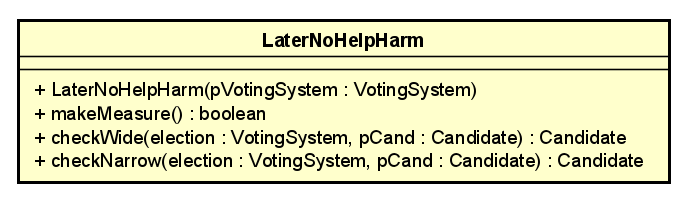
\includegraphics[width=0.7\textwidth]{LaterNoHelpHarm}
\end{figure}

\end{centering}
\normalsize

%0000000000000000000000000000000000000000000000000000000000000000000000000000000000
%0000000000000000000000000000000000000000000000000000000000000000000000000000000000
\newpage
\section{References} \label{References}
%0000000000000000000000000000000000000000000000000000000000000000000000000000000000
%0000000000000000000000000000000000000000000000000000000000000000000000000000000000

\printbibliography[title={\tiny{\textcolor{white}{\cite{polcomp}\cite{anes}\cite{cses}\cite{ideahand}}}}]

\end{document}